\documentclass[11pt]{amsart}

\usepackage[T1]{fontenc}
\usepackage{lmodern}
\usepackage{amssymb,amsmath,amsthm,mathtools}
\usepackage[margin=1.15in]{geometry}
\usepackage{booktabs}
\usepackage{enumitem}
\usepackage{tikz}
\usetikzlibrary{arrows.meta,positioning,calc}
\usepackage{cite}
\usepackage[hidelinks]{hyperref}

\newtheorem{theorem}{Theorem}[section]
\newtheorem{proposition}[theorem]{Proposition}
\newtheorem{lemma}[theorem]{Lemma}
\newtheorem{corollary}[theorem]{Corollary}
\theoremstyle{definition}
\newtheorem{definition}[theorem]{Definition}
\theoremstyle{remark}
\newtheorem{remark}[theorem]{Remark}

\numberwithin{equation}{section}
\emergencystretch=2em

\newcommand{\eps}{\varepsilon}
\newcommand{\iv}[1]{[\,#1\,]}
\newcommand{\en}{\mathrm{en}}
\newcommand{\ex}{\mathrm{ex}}
\newcommand{\nxt}{\mathrm{next}}
\newcommand{\prv}{\mathrm{prev}}
\newcommand{\cost}{\mathrm{cost}}
\newcommand{\owed}{\mathrm{owed}}
\newcommand{\mis}{\mathrm{mis}}
\newcommand{\viol}{\mathrm{viol}}
\newcommand{\Aux}{\mathrm{Aux}}
\newcommand{\pc}{p_{\mathrm{c}}}
\newcommand{\Gh}{\widehat{G}}
\newcommand{\Th}{\widehat{T}}
\newcommand{\cF}{\mathcal{F}}

\begin{document}

\title[A 63/62 inapproximability bound for asymmetric TSP]{A $63/62$ inapproximability bound for the\\ asymmetric traveling salesman problem}

\author{Jizhou Guo}
\email{mitsuha2021b@gmail.com}

\date{October 10, 2026}

\subjclass[2020]{Primary 68Q17; Secondary 68W25, 90C27, 05C20, 05C45}
\keywords{asymmetric traveling salesman problem, hardness of approximation, gadget reduction, bi-wheel amplifier, weighted amplifier, computer-assisted proof}

\begin{abstract}
We prove that for every $\eps>0$ it is NP-hard to approximate the asymmetric (directed) metric traveling salesman problem within a factor of $63/62-\eps$. This improves the bound $75/74$ of Karpinski, Lampis and Schmied (2013), which, to our knowledge, was the best previously known inapproximability bound for this problem. We combine their directed reduction with the weighted bi-wheel amplifiers that Chleb\'{\i}k and Chleb\'{\i}kov\'a (2019) introduced for the symmetric problem. Forced edges of matched checker pairs get weight $1$ and wheel arcs weight $1/2$, so that a matched pair costs $3/2$, and each three-variable equation is simulated by a new module with three auxiliary vertices and $18$ arcs, whose minimum unit cost for an honest profile is $17/2$ if the equation is satisfied and $19/2$ otherwise. This gives a cost of $31$ per three-variable equation against a gap of $1/2$. The weighted amplifiers come from a theorem of Chleb\'{\i}k and Chleb\'{\i}kov\'a whose published proof is a sketch; their bound $117/116$ for the symmetric problem depends on it in the same way. We therefore also prove the bound $73/72$ with an unweighted variant that uses only the amplifiers of Karpinski, Lampis and Schmied and a new module with $10$ vertices and $14$ arcs. In both cases soundness reduces to finite properties of the module: a Hamiltonian path through the module that visits exactly the contacts set to false exists if and only if the equation is satisfied, and in the weighted case the module cannot be covered by two paths to its exit, one from its entry and one from a true contact. The proofs of the two inapproximability theorems are given by hand, and the finite module properties and cost calculations used in them are also checked by short ancillary programs. In the soundness analysis each violated cycle equation is charged to one of its endpoints, so that every variable is decoded from its own gadget; this also corrects two steps in the analysis of Karpinski, Lampis and Schmied.
\end{abstract}

\maketitle

%======================================================================
\section{Introduction}\label{sec:intro}
%======================================================================

In the \emph{asymmetric traveling salesman problem} (ATSP) we are given a finite set $V$ and distances $d\colon V\times V\to\mathbb{Q}_{\geq0}$ satisfying the triangle inequality $d(u,w)\le d(u,v)+d(v,w)$, but not necessarily $d(u,v)=d(v,u)$; the task is to find a Hamiltonian cycle $v_1\to v_2\to\dots\to v_n\to v_1$ minimizing $\sum_i d(v_i,v_{i+1})$ (indices modulo $n$). The symmetric metric TSP is the special case $d(u,v)=d(v,u)$. Without the triangle inequality neither problem can be approximated within any factor unless $\mathrm{P}=\mathrm{NP}$, so throughout ``ATSP'' means the metric version.

\subsection*{Algorithms}
For ATSP, Asadpour, Goemans, M\k{a}dry, Oveis Gharan and Saberi \cite{AGMOS10} gave an $O(\log n/\log\log n)$-approximation. Svensson, Tarnawski and V\'egh \cite{STV20} obtained a constant-factor approximation algorithm. Traub and Vygen improved the ratio to $22+\eps$ \cite{TV22} and then to $17+\eps$ \cite{TV24} (see \cite{Vyg26}), and a recent preprint of Vygen \cite{Vyg26} reports a ratio below $15$. For the symmetric metric TSP, Christofides \cite{Chr76} gave a $3/2$-approximation, and Karlin, Klein and Oveis Gharan \cite{KKO21} gave a randomized algorithm with expected approximation ratio $3/2-\eta$ for some $\eta>10^{-36}$.

\subsection*{Hardness of approximation}
Papadimitriou and Yannakakis \cite{PY93} showed that the TSP with distances one and two is MAX SNP-hard, which together with the PCP theorem \cite{ALMSS98} rules out a polynomial-time approximation scheme unless $\mathrm{P}=\mathrm{NP}$. Explicit constants followed. Engebretsen \cite{Eng03} proved $5381/5380$ for the symmetric problem. Papadimitriou and Vempala \cite{PV06} proved $220/219$ for the symmetric problem and $117/116$ for ATSP, and Lampis \cite{Lam12} proved $185/184$ for the symmetric problem. Karpinski, Lampis and Schmied \cite{KLS15} (henceforth KLS) proved $123/122$ for the symmetric problem and $75/74$ for ATSP. For the symmetric problem, Chleb\'{\i}k and Chleb\'{\i}kov\'a \cite{CC19,CC22} introduced weighted amplifiers and improved the bound to $117/116$, and Nagda, Raghavan and Thakurta \cite{NRT26} improved it further to $111/110$. They kept the reduction of \cite{CC22} and replaced only its equation gadget, which they found with the AlphaEvolve code-mutation agent. The constructions of \cite{CC22,NRT26} are for undirected graphs, and these papers do not state a bound for ATSP. Since symmetric TSP is a special case of ATSP, bounds for the symmetric problem also hold for ATSP, but all of these are smaller than $75/74$. As far as we know, $75/74$ has remained the best inapproximability bound for ATSP; it is the bound listed in the monograph of Traub and Vygen \cite[\S17.1]{TV24} and in the survey of Saller, Koehler and Karrenbauer \cite{SKK25}.

\subsection*{Our results}

\begin{theorem}\label{thm:main}
For every constant $\eps>0$ it is NP-hard to approximate ATSP within a factor of $63/62-\eps$. More precisely, there is a polynomial-time reduction from an NP-complete problem to pairs $(\mathcal{I},\kappa)$, where $\mathcal{I}$ is an ATSP instance with rational distances and $\kappa$ is a rational number, such that yes-instances are mapped to pairs with $\mathrm{OPT}(\mathcal{I})\le\kappa$ and no-instances to pairs with $\mathrm{OPT}(\mathcal{I})\ge(63/62-\eps)\,\kappa$.
\end{theorem}

\begin{corollary}\label{cor:main}
For every fixed rational number $r<63/62$, there is no polynomial-time $r$-approximation algorithm for ATSP unless $\mathrm{P}=\mathrm{NP}$.
\end{corollary}

The restriction to rational $r$ is immaterial: an $r$-approximation algorithm is also an $r'$-approximation algorithm for every rational $r'\in[r,63/62)$. Note that $63/62-75/74=3/1147$.

\begin{theorem}[An unweighted variant]\label{thm:unweighted}
The statement of Theorem~\ref{thm:main} holds with $73/72$ in place of $63/62$, for a reduction whose only external ingredient is the source theorem of KLS (Theorem~\ref{thm:hybrid} below), the same source as for the bound $75/74$.
\end{theorem}

\subsection*{Dependence on the source theorems}
Theorem~\ref{thm:main} uses the weighted bi-wheel amplifiers of Chleb\'{\i}k and Chleb\'{\i}kov\'a: by \cite[Theorem~5]{CC22}, for every sufficiently large $k$ there is a bi-wheel with $k$ contacts and $10k$ checkers on each of its two cycles that is an amplifier when its cycle edges have weight $1/2$ and its matching edges weight $1$ (see Section~\ref{sec:source}). The published proof of this theorem \cite[\S5]{CC22} is a sketch. It chooses the matching at random, states some properties of minimal bad sets and refers for their derivation to the analysis of wheel amplifiers in \cite{CC03}, which, it says, extends in a straightforward way to weighted bi-wheels; the outcome of the final union bound is stated without the computation. We use \cite[Theorem~5]{CC22} as published. The bound $117/116$ of Chleb\'{\i}k and Chleb\'{\i}kov\'a for the symmetric problem depends on the same theorem, and so does the bound $111/110$ of \cite{NRT26}, which uses their reduction. Theorem~\ref{thm:unweighted} avoids this dependence. It uses only the unweighted bi-wheel amplifiers of KLS \cite[Theorem~1]{KLS15}, whose amplification property KLS derive from the analysis of wheel amplifiers by Berman and Karpinski \cite{BK01}; this is the source on which the bound $75/74$ rests.

\subsection*{Approach}
We follow the directed reduction of KLS \cite[\S6]{KLS15}. It starts from a bounded-occurrence system of linear equations modulo~$2$, a \emph{bi-wheel Hybrid instance}, obtained from H\aa{}stad's theorem \cite{Has01} with bi-wheel amplifiers (a variant of the wheel amplifiers of Berman and Karpinski \cite{BK99,BK01}). The variables of the $m$ three-variable equations are \emph{contacts} on bi-wheels, whose other variables, the \emph{checkers}, are linked by two-variable ``matching'' and ``cycle'' equations. In the source of KLS there are $9m$ matching and $21m$ cycle equations, and it is NP-hard to distinguish instances in which at most $\eps m$ equations can be violated from instances in which at least $(1/2-\eps)m$ must be violated (Theorem~\ref{thm:hybrid}). KLS build a directed graph in which each matching equation is simulated by a pair of vertices of local cost~$3$, the cycle equations cost nothing extra, and each three-variable equation is simulated by a gadget of local cost $10$ (up to a small additive term $2\lambda$). This gives $9\cdot3+10=37$ per three-variable equation, and every violated equation costs at least one extra unit. Hence the threshold is $(37+\tfrac12)/37=75/74$.

\emph{The unweighted variant.} For Theorem~\ref{thm:unweighted} we replace only the three-variable gadget, by a module of local cost $9$ in which every violated equation still costs at least one extra unit. In both gadgets every vertex except one port has only outgoing arcs of weight $1$, so the local cost is at least the number of vertices minus one; the KLS gadget has $11$ vertices, ours has $10$ (Table~\ref{tab:arcs} and Figure~\ref{fig:gadget}). To save a vertex the new gadget uses arcs between different contact blocks and between contacts and ports, which do not occur in the KLS gadget.

\emph{The weighted construction.} For Theorem~\ref{thm:main} we use the source of Chleb\'{\i}k and Chleb\'{\i}kov\'a \cite[Theorems~3 and~5]{CC22}. It has $10$ instead of $6$ checkers between consecutive contacts, hence $15m$ matching and $33m$ cycle equations, but a cycle equation has weight $1/2$; the gap is again $1/2$ per three-variable equation, now for the total weight of the violated equations (Theorem~\ref{thm:ccsource}). In the directed reduction we give the forced edge of a matched pair weight $1$ and every wheel arc weight $1/2$, so a matched pair costs $3/2$ instead of $3$, while one unit of excess cost still pays for a violated matching equation (weight $1$) or for two mismatched cycle equations (weight $1/2$ each). Module arcs that leave a contact also get weight $1/2$, so a true contact costs $3/2$ instead of $2$. A new module with three auxiliary vertices and $18$ arcs (Table~\ref{tab:warcs} and Figure~\ref{fig:wgadget}) has minimum unit cost $17/2$ for an honest profile of a satisfied equation and $19/2$ for an honest profile of a violated one. The two thresholds are
\[
\frac{9\cdot3+9+\tfrac12}{9\cdot3+9}=\frac{36+\tfrac12}{36}=\frac{73}{72}
\qquad\text{and}\qquad
\frac{15\cdot\tfrac32+\tfrac{17}{2}+\tfrac12}{15\cdot\tfrac32+\tfrac{17}{2}}=\frac{31+\tfrac12}{31}=\frac{63}{62}.
\]

\emph{Parity and two-start properties.} We derive soundness from finite properties of the block digraphs of the modules. One is the \emph{parity property} (Lemmas~\ref{lem:parity} and~\ref{lem:wparity}): a Hamiltonian path from the entry port to the exit port through the auxiliary vertices and exactly the contacts that are set to false exists if and only if an even number of contacts is false, that is, if and only if the equation $x\oplus y\oplus z=1$ is satisfied. In the unweighted setting the decoding lemma (Lemma~\ref{lem:module}) shows that, together with an exact cost identity for the contact vertices (Lemma~\ref{lem:contact}) and global connectivity, the parity property forces every violated equation to be paid for. In the weighted setting a true contact can emit a module arc at an extra cost of only $1/2$. This opens a second way to traverse a module cheaply: by two paths to the exit port, one from the entry port and one from a true contact. The \emph{two-start property} of the weighted module (Lemma~\ref{lem:wparity}(b)) excludes this, and the same decoding lemma applies.

\subsection*{The soundness analysis of the two-variable part}
We keep the KLS gadgets for the matching and cycle equations (with the weights halved in the weighted setting), but we present the decoding of the checker variables differently. Each violated cycle equation is charged to an endpoint whose decoded value disagrees with the usage of the wheel arc that represents this equation. With this per-endpoint charging, the value of every variable depends only on the arcs at its own gadget, and each gadget can be analyzed on its own (Lemmas~\ref{lem:charging}, \ref{lem:pair} and~\ref{lem:module}). This also corrects two steps of \cite[\S6.3]{KLS15}. When both checkers of a matched pair are traversed honestly with value $1$, the local cost is at least $5$ and not at least $6$ as stated there. The resulting credit of $2$ still pays for the single violated equation (Remark~\ref{rem:kls}). The rule given there for a matched pair with exactly one dishonest checker (assign it the value $0$) is justified relative to the values of the neighboring variables. If a neighboring contact is assigned a value that disagrees with the usage of the wheel arc between them, which the decoding of contacts may require, this rule can leave two violated equations against a credit of one. Choosing the values of both checkers from the arcs at the pair alone, together with the per-endpoint charging, repairs this (Lemma~\ref{lem:pair}). Both points concern the presentation of the argument, and Lemma~\ref{lem:pair} applies verbatim to the matched pairs of the KLS construction.

\subsection*{Computer search and verification}
Both modules were found by computer searches with SAT encodings of the parity property and, for the weighted module, of the two-start property. The proofs of the two inapproximability theorems use the explicit arc sets in Tables~\ref{tab:arcs} and~\ref{tab:warcs}. The finite module properties, completeness walks and cost calculations used in these proofs are proved in the text and also checked by standalone programs in the ancillary files. The local lemmas of the soundness proof are proved for arbitrary multiplicities and additionally checked by exhaustive enumeration over the finite ranges specified in Section~\ref{sec:computation}.

\subsection*{Organization}
Section~\ref{sec:prelim} fixes notation and states the two source problems. Section~\ref{sec:construction} describes the reduction and the two modules. Section~\ref{sec:parity} proves the parity and two-start properties. Section~\ref{sec:completeness} proves completeness and Section~\ref{sec:soundness} proves soundness, for both settings at once. Section~\ref{sec:proofmain} proves Theorems~\ref{thm:main} and~\ref{thm:unweighted}, and Section~\ref{sec:computation} describes the computations and the ancillary files and contains some remarks.

%======================================================================
\section{Preliminaries}\label{sec:prelim}
%======================================================================

\subsection{Tours}
All graphs are directed multigraphs with positive rational arc weights. For a multiset $T$ of arcs of a digraph $G$ and a vertex $v$, let $\mathrm{out}_T(v)$ and $\mathrm{in}_T(v)$ be the numbers of arcs of $T$ (with multiplicity) leaving and entering $v$. The multiset $T$ is \emph{balanced} if $\mathrm{out}_T(v)=\mathrm{in}_T(v)$ for all $v$. Following KLS \cite[\S2]{KLS15}, a \emph{tour} of $G$ is a balanced multiset $T$ of arcs of $G$ such that every vertex of $G$ is incident with an arc of $T$ and the graph $(V(G),T)$ is weakly connected. Its cost is $\cost(T)=\sum_{a\in T}w(a)$, counted with multiplicity. For $V'\subseteq V(G)$, the \emph{local cost} of $V'$ is the total weight of the arcs of $T$ whose tail lies in $V'$:
\[
c_T(V')=\sum_{(x,y)\in T,\ x\in V'}w(x,y).
\]
If $V_1,\dots,V_k$ partition $V(G)$ then $\cost(T)=\sum_i c_T(V_i)$.

\begin{proposition}[{cf.\ \cite[\S2]{KLS15}}]\label{prop:tours}
Let $G$ be a strongly connected digraph with positive arc weights, and let $d_G$ be its shortest-path distance. Then $(V(G),d_G)$ is an ATSP instance, and its optimum equals the minimum cost of a tour of $G$.
\end{proposition}

\begin{proof}
$d_G$ satisfies the triangle inequality. Replacing each step of a Hamiltonian cycle of $(V(G),d_G)$ by a shortest path of $G$ gives a tour of $G$ of the same cost. Conversely, a tour of $G$ is a connected balanced multigraph, so it has a closed Eulerian walk through all vertices; listing the vertices in the order of their earliest visits gives a Hamiltonian cycle whose cost, by the triangle inequality, is at most the cost of the tour.
\end{proof}

\subsection{The source problems}\label{sec:source}
We use the following special systems of weighted equations modulo $2$, constructed by KLS \cite[\S4]{KLS15} in the unweighted case and by Chleb\'{\i}k and Chleb\'{\i}kov\'a \cite[\S\S2--3]{CC22} in the weighted case.

\begin{definition}\label{def:hybrid}
Let $g\ge1$ be an integer and $\pc\in(0,1]$ a rational number. A \emph{bi-wheel with gap $g$} consists of two disjoint cycles $Q^u$ and $Q^n$ of the same length $(g+1)n$ ($n\ge1$), whose vertices are Boolean variables, together with a perfect matching between the checkers of $Q^u$ and the checkers of $Q^n$. Here, on each cycle, the variables at positions $g+1,2(g+1),\dots,(g+1)n$ are the \emph{contacts} and the remaining $gn$ variables are the \emph{checkers}. A \emph{bi-wheel Hybrid instance with gap $g$ and cycle weight $\pc$} consists of $\nu$ variable-disjoint bi-wheels with gap $g$ together with $m$ equations of the form $x\oplus y\oplus z=1$ over three distinct contacts, the \emph{parity equations}, such that every contact occurs in exactly one parity equation and no checker occurs in any parity equation. Its equations, with their weights, are:
\begin{itemize}[leftmargin=2em]
\item a \emph{cycle equation} $y\oplus z=0$ of weight $\pc$ for every edge $\{y,z\}$ of a cycle $Q^u$ or $Q^n$;
\item a \emph{matching equation} $p\oplus q=1$ of weight $1$ for every edge $\{p,q\}$ of a matching;
\item the $m$ parity equations, of weight $1$.
\end{itemize}
For an assignment $\sigma$, the \emph{violated weight} $\viol_I(\sigma)$ is the total weight of the equations violated by $\sigma$. An assignment is \emph{consistent} if on every bi-wheel all variables of $Q^u$ take one value and all variables of $Q^n$ take the other value.
\end{definition}

There are $3m$ contacts and hence $3gm$ checkers, $\frac{3g}{2}m$ matching equations and $3(g+1)m$ cycle equations: $18m$, $9m$ and $21m$ for $g=6$, and $30m$, $15m$ and $33m$ for $g=10$. Every variable occurs in exactly three equations. A consistent assignment satisfies all cycle and matching equations, so its violated weight is the number of parity equations it violates.

\begin{theorem}[Karpinski, Lampis and Schmied]\label{thm:hybrid}
For all constants $\eps,\delta>0$ there is a polynomial-time reduction from an NP-complete problem to bi-wheel Hybrid instances $I$ with gap $6$ and cycle weight $1$, with $m$ parity equations and $\nu\le\delta m$ bi-wheels, such that:
\begin{enumerate}[label=\textup{(\roman*)},leftmargin=2.2em]
\item if the input is a yes-instance, some consistent assignment of $I$ violates at most $\eps m$ equations;
\item if the input is a no-instance, every assignment of $I$ violates at least $(1/2-\eps)m$ equations.
\end{enumerate}
\end{theorem}

This is \cite[Theorem~3]{KLS15} (with right-hand side $b=1$), applied as in the proof of \cite[Theorem~5]{KLS15}. There, every equation of the H\aa{}stad instance is repeated a sufficiently large constant number of times before the bi-wheel construction, which makes $\nu/m$ smaller than any fixed $\delta>0$. The bi-wheels have constant size and are found in constant time \cite[proof of Theorem~3]{KLS15}. That the assignment in~(i) can be taken consistent is part of the proof of \cite[Theorem~3]{KLS15} and is used in the same way in \cite[Lemma~3]{KLS15}.

\begin{theorem}[Chleb\'{\i}k and Chleb\'{\i}kov\'a]\label{thm:ccsource}
For all constants $\eps\in(0,1/4)$ and $\delta>0$ there is a polynomial-time reduction from an NP-complete problem to bi-wheel Hybrid instances $I$ with gap $10$ and cycle weight $1/2$, with $m$ parity equations and $\nu\le\delta m$ bi-wheels, such that:
\begin{enumerate}[label=\textup{(\roman*)},leftmargin=2.2em]
\item if the input is a yes-instance, some consistent assignment of $I$ violates at most $\eps m$ equations;
\item if the input is a no-instance, every assignment $\sigma$ of $I$ has $\viol_I(\sigma)\ge(1/2-\eps)m$.
\end{enumerate}
\end{theorem}

Theorem~\ref{thm:ccsource} is \cite[Theorem~3]{CC22} with $b=1$ and the amplifier of \cite[Theorem~5]{CC22}, as follows. By \cite[Theorem~2]{CC22} (the fixed-occurrence form of H\aa{}stad's theorem, see \cite{CC03}), for every fixed $k\ge k(\eps)$ it is NP-hard, given a system of $m$ equations $x\oplus y\oplus z=1$ over literals in which every variable occurs exactly $k$ times unnegated and $k$ times negated, to decide whether some assignment satisfies at least $(1-\eps)m$ equations or every assignment satisfies at most $(1/2+\eps)m$ of them. By \cite[Theorem~5]{CC22}, for every sufficiently large $k$ there is a $(2k,11)$-bi-wheel in the sense of \cite[Definition~2]{CC22}, with contacts at the positions $11,22,\dots,11k$ of both cycles (so it has gap $10$ in the sense of Definition~\ref{def:hybrid}), which is an amplifier \cite[Definition~1]{CC22} when its cycle edges have weight $1/2$ and its matching edges weight $1$. Fix $k\ge3/(2\delta)$ so large that both statements apply. \cite[Theorem~5]{CC22} is an existence statement, proved with a random matching. For fixed $k$, however, the bi-wheel has $22k$ vertices, so the reduction can find one deterministically by exhaustive search over the $(10k)!$ matchings, checking the amplifier inequality for all $2^{22k}$ vertex sets; this takes constant time. The construction in the proof of \cite[Theorem~3]{CC22} replaces every variable $x$ by a copy of this bi-wheel, with the unnegated occurrences of $x$ at the contacts of $Q^u$ and the negated ones at the contacts of $Q^n$. This gives a bi-wheel Hybrid instance with gap $10$ and cycle weight $1/2$ in which the $\nu$ variables of the original system give $\nu$ bi-wheels, and $2k\nu=3m$, so $\nu/m=3/(2k)\le\delta$. Part~(ii) is the conclusion of \cite[Theorem~3]{CC22} for no-instances. For part~(i), take an assignment of the original system that satisfies at least $(1-\eps)m$ equations, and give every variable of $Q^u$ in the bi-wheel of $x$ the value of $x$ and every variable of $Q^n$ the opposite value. This is the \emph{standard} assignment of \cite[\S2]{CC22}. It is consistent, so it satisfies all cycle and matching equations, and since a negated occurrence of $x$ sits on $Q^n$, it violates exactly the parity equations that come from violated equations of the original system, at most $\eps m$ of them. (Alternatively, \cite[\S2]{CC22} shows that the amplifier property converts every assignment into a standard one without increasing the violated weight; \cite[Lemma~1]{CC22} uses the yes-case in this form.)

%======================================================================
\section{The construction}\label{sec:construction}
%======================================================================

Throughout the rest of the paper we fix one of the two settings of Table~\ref{tab:params}. The \emph{unweighted setting} is the construction of KLS with our unweighted module; it is used for Theorem~\ref{thm:unweighted}. The \emph{weighted setting} is used for Theorem~\ref{thm:main}.

\begin{table}[ht]
\centering
\begin{tabular}{@{}lcc@{}}
\toprule
 & unweighted setting & weighted setting\\
\midrule
source theorem & Theorem~\ref{thm:hybrid} (KLS) & Theorem~\ref{thm:ccsource} (CC)\\
gap $g$ (checkers between consecutive contacts) & $6$ & $10$\\
cycle weight $\pc$ (weight of a wheel arc) & $1$ & $1/2$\\
weight of the forced edge of a matched pair, $2\pc$ & $2$ & $1$\\
matched pairs per parity equation, $3g/2$ & $9$ & $15$\\
auxiliary vertices of a module & $A,B$ & $A,B,C$\\
module arcs & $14$ (Table~\ref{tab:arcs}) & $18$ (Table~\ref{tab:warcs})\\
module baseline $\theta$ & $9$ & $17/2$\\
baseline per parity equation, $\Theta=\frac{3g}{2}\cdot3\pc+\theta$ & $36$ & $31$\\
connector cost $\zeta$ & $6$ & $5/2$\\
normalization error (Lemma~\ref{lem:normalize}) & $42m/L$ & $36m/L$\\
threshold $(\Theta+\frac12)/\Theta$ & $73/72$ & $63/62$\\
\bottomrule
\end{tabular}
\medskip
\caption{The two settings. In both, contact forced edges have weight $1$, portals have weight $\lambda$, module arcs leaving a contact have weight $\pc$, and all other module arcs have weight $1$.}
\label{tab:params}
\end{table}

Fix a bi-wheel Hybrid instance $I$ with gap $g$ and cycle weight $\pc$, a rational $\lambda>0$ and an integer $L\ge2$. We describe a graph $\Gh=\Gh(I,\lambda)$ with \emph{forced edges} and then the weighted digraph $G=G(I,\lambda,L)$ obtained by replacing forced edges by long paths, as in \cite{Lam12,KLS15}. In the unweighted setting everything except the parity modules (Section~\ref{sec:module}) is the construction of KLS \cite[\S6.1]{KLS15}; in the weighted setting we also change the weights of the forced edges of matched pairs and of the wheel arcs. We describe both in a uniform notation.

\subsection{Wheels and matching pairs}\label{sec:wheels}
Orient each cycle of each bi-wheel cyclically and write $\nxt(y)$ and $\prv(y)$ for the successor and predecessor of a variable $y$ on its cycle. For a checker $p$ let $\pi(p)$ be the checker matched to $p$; it lies on the other cycle of the same bi-wheel.

The graph $\Gh$ has a root vertex $s$ and the following vertices for the variables: one vertex for each checker $p$ (also denoted $p$), and two vertices $c^{r}$ and $c^{l}$ for each contact $c$. For each variable $y$ we define an \emph{entry vertex} $\en(y)$ and an \emph{exit vertex} $\ex(y)$:
\[
\en(p)=p,\quad \ex(p)=\pi(p)\quad\text{for a checker }p;\qquad \en(c)=c^{r},\quad \ex(c)=c^{l}\quad\text{for a contact }c.
\]
Thus a matched pair $\{p,\pi(p)\}$ satisfies $\ex(p)=\en(\pi(p))$ and $\ex(\pi(p))=\en(p)$.

\begin{itemize}[leftmargin=2em]
\item \emph{Forced edges of the variables.} For each matching equation $p\oplus\pi(p)=1$ there is a bidirected forced edge $\{p,\pi(p)\}$ of weight $2\pc$. For each contact $c$ there is a bidirected forced edge $\{c^r,c^l\}$ of weight $1$.
\item \emph{Wheel arcs.} For each cycle equation $e=\{y,z\}$ with $z=\nxt(y)$ there is an ordinary arc $\rho_e=(\ex(y),\en(z))$ of weight $\pc$; we say that $\rho_e$ \emph{represents} $e$.
\end{itemize}
Every checker vertex $p$ is the head of exactly one wheel arc, namely $\rho_{\{\prv(p),p\}}$, and the tail of exactly one wheel arc, namely $\rho_{\{\pi(p),\nxt(\pi(p))\}}$. It is incident with no other arcs except its forced edge. For a contact $c$, the vertex $c^r$ is the head of exactly one wheel arc, $\rho_{\{\prv(c),c\}}$, and $c^l$ is the tail of exactly one wheel arc, $\rho_{\{c,\nxt(c)\}}$.

The \emph{intended traversal} of a cycle $Q$ is the closed walk that, for every $y\in Q$ in cyclic order, traverses the forced edge $\en(y)\to\ex(y)$ followed by the wheel arc $\ex(y)\to\en(\nxt(y))$. It visits all checkers of the bi-wheel, because every checker of the other cycle is $\ex(y)$ for some checker $y\in Q$. It also visits the contacts of $Q$, but not those of the other cycle. It traverses the forced edge of each contact $c\in Q$ in the direction $c^r\to c^l$ (``true''). In the construction below, a false contact is instead visited by the parity module in the direction $c^l\to c^r$.

\subsection{The parity modules}\label{sec:module}
For each parity equation $j$, fix an order $(X_j,Y_j,Z_j)$ of its three contacts. Add new vertices $s_j,t_j$ and the \emph{auxiliary vertices} of the module, which form the set $\Aux_j=\{A_j,B_j\}$ in the unweighted and $\Aux_j=\{A_j,B_j,C_j\}$ in the weighted setting. Add the \emph{portals}, which are ordinary arcs $s\to s_j$ and $t_j\to s$ of weight $\lambda$, and the \emph{module arcs} listed in Table~\ref{tab:arcs} ($14$ arcs, unweighted setting) or Table~\ref{tab:warcs} ($18$ arcs, weighted setting). We use \emph{block notation}: an arc written as entering a contact $c\in\{X_j,Y_j,Z_j\}$ ends at $c^l$, and an arc written as leaving $c$ starts at $c^r$. A module arc leaving a contact has weight $\pc$, and every other module arc has weight $1$; so in the unweighted setting all module arcs have weight $1$. We abbreviate $s_j,t_j,A_j,B_j,C_j,X_j,Y_j,Z_j$ as $s,t,A,B,C,X,Y,Z$ inside a module; the root is always called ``the root $s$'' when there is a risk of confusion. Note that no module arc enters $s_j$ or leaves $t_j$, and that no module arc is incident with a checker. So the only arc entering $s_j$ and the only arc leaving $t_j$ are the portals.

\begin{table}[ht]
\centering
\begin{tabular}{@{}lll@{}}
\toprule
tail & heads (block notation) & arcs of $\Gh$ \\
\midrule
$s_j$ & $B,\ Z$ & $s_j\to B_j,\ s_j\to Z_j^l$\\
$A$ & $B,\ X,\ t_j$ & $A_j\to B_j,\ A_j\to X_j^l,\ A_j\to t_j$\\
$B$ & $A,\ Y$ & $B_j\to A_j,\ B_j\to Y_j^l$\\
$X$ & $A,\ Y,\ Z$ & $X_j^r\to A_j,\ X_j^r\to Y_j^l,\ X_j^r\to Z_j^l$\\
$Y$ & $B,\ X$ & $Y_j^r\to B_j,\ Y_j^r\to X_j^l$\\
$Z$ & $Y,\ t_j$ & $Z_j^r\to Y_j^l,\ Z_j^r\to t_j$\\
\bottomrule
\end{tabular}
\medskip
\caption{The $14$ module arcs of the unweighted module for the equation $X\oplus Y\oplus Z=1$. All have weight $1$. The same arc set is given in the ancillary file \texttt{parity\_boundary.json} (where $s$ and $t$ denote $s_j$ and $t_j$).}
\label{tab:arcs}
\end{table}

\begin{table}[ht]
\centering
\begin{tabular}{@{}llll@{}}
\toprule
tail & heads (block notation) & arcs of $\Gh$ & weight\\
\midrule
$s_j$ & $A,\ X,\ Y,\ Z$ & $s_j\to A_j,\ s_j\to X_j^l,\ s_j\to Y_j^l,\ s_j\to Z_j^l$ & $1$\\
$A$ & $B,\ X,\ Z$ & $A_j\to B_j,\ A_j\to X_j^l,\ A_j\to Z_j^l$ & $1$\\
$B$ & $A,\ C$ & $B_j\to A_j,\ B_j\to C_j$ & $1$\\
$C$ & $A,\ B,\ t_j$ & $C_j\to A_j,\ C_j\to B_j,\ C_j\to t_j$ & $1$\\
$X$ & $C,\ t_j$ & $X_j^r\to C_j,\ X_j^r\to t_j$ & $1/2$\\
$Y$ & $C,\ t_j$ & $Y_j^r\to C_j,\ Y_j^r\to t_j$ & $1/2$\\
$Z$ & $C,\ t_j$ & $Z_j^r\to C_j,\ Z_j^r\to t_j$ & $1/2$\\
\bottomrule
\end{tabular}
\medskip
\caption{The $18$ module arcs of the weighted module for the equation $X\oplus Y\oplus Z=1$. The same arc set is given in the ancillary file \texttt{half\_contact\_\allowbreak 3aux\_\allowbreak candidate.json}.}
\label{tab:warcs}
\end{table}

\begin{figure}[ht]
\centering
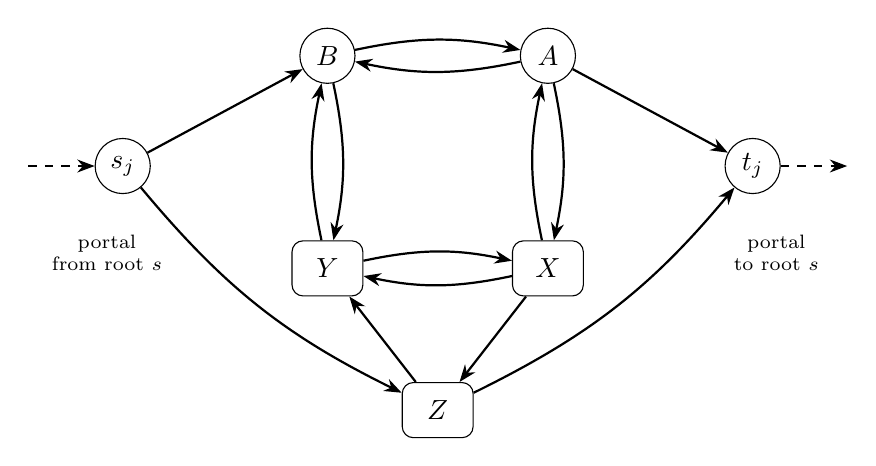
\begin{tikzpicture}[
  >={Stealth[length=2.2mm]},
  v/.style={circle,draw,minimum size=7mm,inner sep=0pt},
  blk/.style={rectangle,rounded corners,draw,minimum width=9mm,minimum height=7mm,inner sep=1pt},
  every edge/.style={draw,->,thick},
  lab/.style={font=\scriptsize}
]
\node[v] (s) at (0,0.1) {$s_j$};
\node[v] (t) at (8,0.1) {$t_j$};
\node[v] (B) at (2.6,1.5) {$B$};
\node[v] (A) at (5.4,1.5) {$A$};
\node[blk] (Y) at (2.6,-1.2) {$Y$};
\node[blk] (X) at (5.4,-1.2) {$X$};
\node[blk] (Z) at (4,-3.0) {$Z$};
\path (s) edge (B)
      (s) edge[bend right=12] (Z)
      (A) edge[bend left=12] (B)
      (B) edge[bend left=12] (A)
      (A) edge[bend left=12] (X)
      (X) edge[bend left=12] (A)
      (A) edge (t)
      (B) edge[bend left=12] (Y)
      (Y) edge[bend left=12] (B)
      (X) edge[bend left=12] (Y)
      (Y) edge[bend left=12] (X)
      (X) edge (Z)
      (Z) edge (Y)
      (Z) edge[bend right=12] (t);
\node[lab,align=center] at (-0.2,-1.0) {portal\\ from root $s$};
\draw[->,dashed] (-1.2,0.1) -- (s);
\draw[->,dashed] (t) -- (9.2,0.1);
\node[lab,align=center] at (8.3,-1.0) {portal\\ to root $s$};
\end{tikzpicture}

\bigskip

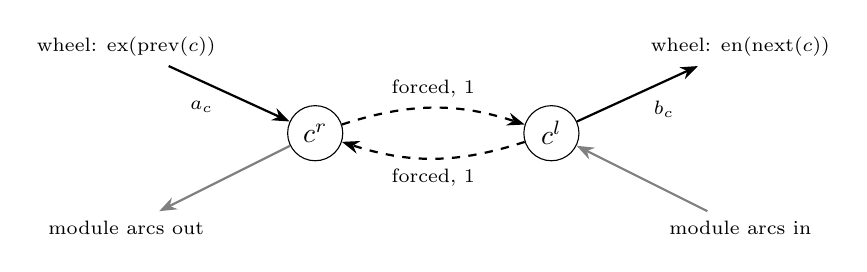
\begin{tikzpicture}[
  >={Stealth[length=2.2mm]},
  v/.style={circle,draw,minimum size=7mm,inner sep=0pt},
  lab/.style={font=\scriptsize},
]
\node[v] (cr) at (0,0) {$c^r$};
\node[v] (cl) at (3,0) {$c^l$};
\draw[->,thick,dashed] (cr) to[bend left=18] node[above,lab] {forced, $1$} (cl);
\draw[->,thick,dashed] (cl) to[bend left=18] node[below,lab] {forced, $1$} (cr);
\node[lab,align=center] (wi) at (-2.4,1.1) {wheel: $\ex(\prv(c))$};
\node[lab,align=center] (wo) at (5.4,1.1) {wheel: $\en(\nxt(c))$};
\draw[->,thick] (wi) -- node[below left,lab,pos=0.45] {$a_c$} (cr);
\draw[->,thick] (cl) -- node[below right,lab,pos=0.55] {$b_c$} (wo);
\node[lab] (mi) at (5.4,-1.2) {module arcs in};
\node[lab] (mo) at (-2.4,-1.2) {module arcs out};
\draw[->,thick,gray] (mi) -- (cl);
\draw[->,thick,gray] (cr) -- (mo);
\end{tikzpicture}

\bigskip

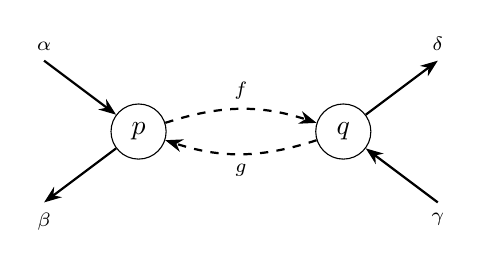
\begin{tikzpicture}[
  >={Stealth[length=2.2mm]},
  v/.style={circle,draw,minimum size=7mm,inner sep=0pt},
  lab/.style={font=\scriptsize},
]
\node[v] (p) at (0,0) {$p$};
\node[v] (q) at (2.6,0) {$q$};
\draw[->,thick,dashed] (p) to[bend left=18] node[above,lab] {$f$} (q);
\draw[->,thick,dashed] (q) to[bend left=18] node[below,lab] {$g$} (p);
\draw[<-,thick] (p) -- ++(-1.2,0.9) node[above,lab] {$\alpha$};
\draw[->,thick] (p) -- ++(-1.2,-0.9) node[below,lab] {$\beta$};
\draw[<-,thick] (q) -- ++(1.2,-0.9) node[below,lab] {$\gamma$};
\draw[->,thick] (q) -- ++(1.2,0.9) node[above,lab] {$\delta$};
\end{tikzpicture}
\caption{Top: the block graph of the unweighted module (Table~\ref{tab:arcs}). A rectangle $c\in\{X,Y,Z\}$ stands for the pair $c^l,c^r$: arcs drawn into $c$ end at $c^l$ and arcs drawn out of $c$ start at $c^r$. Middle: the interface of a contact $c$ (in both settings), with the multiplicities $a_c,b_c$ of its two wheel arcs used in Lemma~\ref{lem:contact}. The wheel traverses $c^r\to c^l$ (true); the module traverses $c^l\to c^r$ (false). Bottom: a matched pair $\{p,q\}$ of checkers with the multiplicities used in Lemma~\ref{lem:pair}; $\alpha,\gamma$ are the wheel arcs entering $p,q$, $\beta,\delta$ the wheel arcs leaving $p,q$, and $f,g$ count traversals of the forced edge (weight $2\pc$).}
\label{fig:gadget}
\end{figure}

\begin{figure}[ht]
\centering
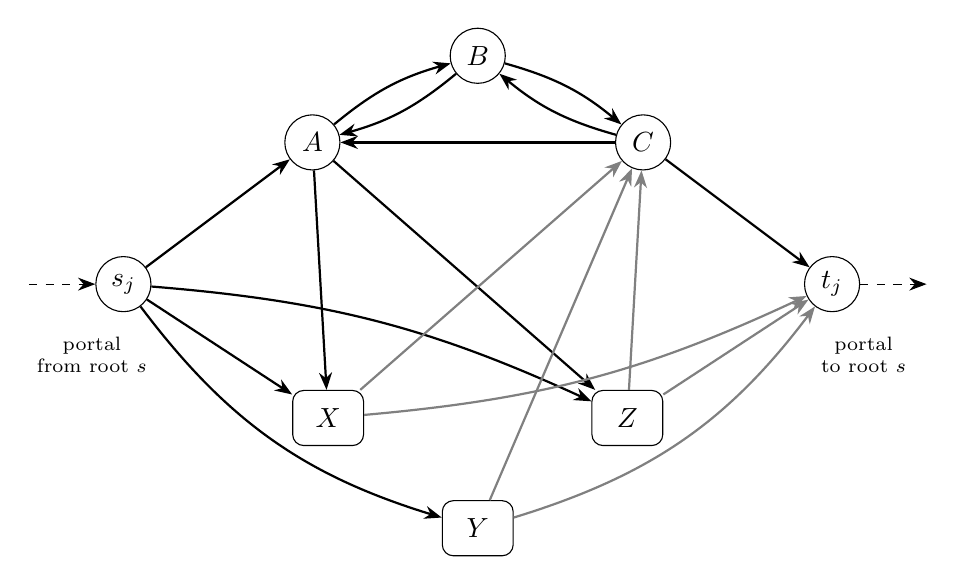
\begin{tikzpicture}[
  >={Stealth[length=2.2mm]},
  v/.style={circle,draw,minimum size=7mm,inner sep=0pt},
  blk/.style={rectangle,rounded corners,draw,minimum width=9mm,minimum height=7mm,inner sep=1pt},
  every edge/.style={draw,->,thick},
  half/.style={gray},
  lab/.style={font=\scriptsize}
]
\node[v] (s) at (0,0) {$s_j$};
\node[v] (t) at (9,0) {$t_j$};
\node[v] (A) at (2.4,1.8) {$A$};
\node[v] (B) at (4.5,2.9) {$B$};
\node[v] (C) at (6.6,1.8) {$C$};
\node[blk] (X) at (2.6,-1.7) {$X$};
\node[blk] (Y) at (4.5,-3.1) {$Y$};
\node[blk] (Z) at (6.4,-1.7) {$Z$};
\path (s) edge (A)
      (s) edge (X)
      (s) edge[bend right=18] (Y)
      (s) edge[bend left=10] (Z)
      (A) edge[bend left=12] (B)
      (B) edge[bend left=12] (A)
      (B) edge[bend left=12] (C)
      (C) edge[bend left=12] (B)
      (C) edge (A)
      (A) edge (X)
      (A) edge (Z)
      (C) edge (t)
      (X) edge[half] (C)
      (Y) edge[half] (C)
      (Z) edge[half] (C)
      (X) edge[half,bend right=10] (t)
      (Y) edge[half,bend right=18] (t)
      (Z) edge[half] (t);
\draw[->,dashed] (-1.2,0) -- (s);
\draw[->,dashed] (t) -- (10.2,0);
\node[lab,align=center] at (-0.4,-0.9) {portal\\ from root $s$};
\node[lab,align=center] at (9.4,-0.9) {portal\\ to root $s$};
\end{tikzpicture}
\caption{The block graph of the weighted module (Table~\ref{tab:warcs}), with the same conventions as in Figure~\ref{fig:gadget}. The gray arcs leave a contact and have weight $1/2$; the black arcs have weight $1$.}
\label{fig:wgadget}
\end{figure}

\subsection{Forced edges and the graph \texorpdfstring{$G$}{G}}\label{sec:forced}
A \emph{tour of $\Gh$} is a balanced, weakly connected multiset $\Th$ of arcs of $\Gh$ covering all vertices, where each forced edge of weight $w$ may be used, any number of times, as an arc of weight $w$ in either of its directions, and every forced edge is used at least once. The portals are ordinary arcs, but every tour uses each of them at least once: $s_j$ is covered and balanced, and its only entering arc is its portal; similarly, the only arc leaving $t_j$ is its portal. For this reason the portals need not be forced.

The digraph $G=G(I,\lambda,L)$ is obtained from $\Gh$ by replacing each forced edge of weight $w$ between $x$ and $y$ by a path $x=z_0,z_1,\dots,z_L=y$ through $L-1$ new \emph{internal} vertices, with the arcs $(z_{i-1},z_i)$ and $(z_i,z_{i-1})$ of weight $w/L$ for $1\le i\le L$. Internal vertices have no other arcs. All other arcs of $\Gh$, including the portals, are kept. Thus $G$ has $1+3gm+6m+(2+|\Aux_j|)m+(L-1)(\frac{3g}{2}+3)m$ vertices, that is, $1+28m+12(L-1)m$ in the unweighted and $1+41m+18(L-1)m$ in the weighted setting, and all weights are positive rationals, so for fixed $\lambda$ and $L$ it can be constructed in polynomial time.

%======================================================================
\section{The parity and two-start properties}\label{sec:parity}
%======================================================================

Let $H$ be the \emph{block digraph} of the module under consideration: its vertex set is $\{s,t\}\cup\Aux\cup\{X,Y,Z\}$, where $\Aux=\{A,B\}$ in the unweighted and $\Aux=\{A,B,C\}$ in the weighted setting, and its arcs are the arcs of Table~\ref{tab:arcs} or Table~\ref{tab:warcs} in block notation. For $F\subseteq\{X,Y,Z\}$ let $H_F$ be the subdigraph induced by $\{s,t\}\cup\Aux\cup F$. A \emph{Hamiltonian port path} of $H_F$ is a directed path from $s$ to $t$ that visits every vertex of $H_F$ exactly once. The module has the \emph{parity property} if, for every $F\subseteq\{X,Y,Z\}$, the digraph $H_F$ has a Hamiltonian port path if and only if $|F|$ is even.

\begin{lemma}[Parity property of the unweighted module]\label{lem:parity}
The unweighted module has the parity property.
\end{lemma}

\begin{proof}
For even $|F|$ the following paths use only arcs of Table~\ref{tab:arcs}:
\[
\begin{aligned}
F&=\emptyset: && sBAt, &\qquad F&=\{X,Y\}: && sBYXAt,\\
F&=\{X,Z\}: && sBAXZt, &\qquad F&=\{Y,Z\}: && sZYBAt.
\end{aligned}
\]
Now let $|F|$ be odd. We list the arcs of $H_F$ that matter and show that no Hamiltonian port path exists.

\emph{$F=\{X\}$.} In $H_F$ the only arc leaving $s$ is $s\to B$ and the only arc leaving $B$ is $B\to A$, so a Hamiltonian port path starts $sBA$. From $A$ it must go to $X$ (going to $t$ would miss $X$), but the only arc leaving $X$ in $H_F$ is $X\to A$.

\emph{$F=\{Y\}$.} The only arc leaving $s$ is $s\to B$. The only arc leaving $Y$ in $H_F$ is $Y\to B$, so $Y$ cannot be visited after $B$; the only arc leaving $A$ other than $A\to B$ is $A\to t$, so $Y$ cannot be visited after $A$ either.

\emph{$F=\{Z\}$.} The only arc entering $Z$ in $H_F$ is $s\to Z$ and the only arc leaving $Z$ is $Z\to t$, so the path would be $sZt$, which misses $A$ and $B$.

\emph{$F=\{X,Y,Z\}$.} The arcs entering $t$ come from $A$ and $Z$, the arcs entering $Z$ come from $s$ and $X$, and the arcs leaving $Z$ go to $Y$ and $t$. Suppose that the path ends with $Z\to t$. Then $Z$ is preceded by $X$ (not by $s$, since the path has $7$ vertices), so the path starts with $s\to B$ and has the form $sB\,\cdot\,\cdot\,XZt$ with $A$ and $Y$ in the two open positions. This needs $A\to Y$ or $Y\to A$, and neither is an arc. Suppose next that the path ends with $A\to t$. Then $Z$ is followed by $Y$. If $Z$ is preceded by $s$, the path is $sZY\,\cdot\,\cdot\,At$ with $B,X$ in the open positions, which needs $B\to X$ or $X\to B$; neither is an arc. If $Z$ is preceded by $X$, the path starts with $s\to B$ and contains the segment $XZY$, so it is $sBXZYAt$, which needs the arc $B\to X$; it does not exist.
\end{proof}

The paths listed for even $|F|$ are in fact the only Hamiltonian port paths. This, and the lemma itself, is also verified by exhaustive enumeration in the ancillary programs \texttt{check\_parity\_ham.py}, \texttt{check\_final.py} and \texttt{check\_tables.py}.

\begin{lemma}[Properties of the weighted module]\label{lem:wparity}
\leavevmode
\begin{enumerate}[label=\textup{(\alph*)},leftmargin=2.2em]
\item The weighted module has the parity property.
\item \textup{(Two-start property.)} Let $c$ and $c'$ be distinct contacts. There are no two directed paths $P_1$ from $s$ to $t$ and $P_2$ from $c'$ to $t$ in $H_{\{c,c'\}}$ that have only $t$ in common and together visit every vertex of $\Aux\cup\{c\}$.
\end{enumerate}
\end{lemma}

\begin{proof}
We use the following facts about Table~\ref{tab:warcs}: (F1) every arc leaving a contact ends at $C$ or $t$; (F2) the arcs entering $t$ come from $C$, $X$, $Y$ and $Z$; (F3) the only arc entering $Y$ is $s\to Y$, and the arcs entering $X$ and $Z$ come from $s$ and $A$; (F4) the only auxiliary vertex that $s$ has an arc to is $A$, and the arcs leaving $B$ go to $A$ and $C$.

(a) For even $|F|$ the following paths use only arcs of Table~\ref{tab:warcs}:
\[
\begin{aligned}
F&=\emptyset: && sABCt, &\qquad F&=\{X,Y\}: && sYCBAXt,\\
F&=\{X,Z\}: && sXCBAZt\ \text{ and }\ sZCBAXt, &\qquad F&=\{Y,Z\}: && sYCBAZt.
\end{aligned}
\]
Now let $|F|$ be odd and suppose that $H_F$ has a Hamiltonian port path. By (F1) every contact on it is followed by $C$ or by $t$. Each of $C$ and $t$ occurs once, so at most two contacts occur, and $|F|=1$, say $F=\{c\}$. By (F2) the predecessor of $t$ is $C$ or $c$. If it is $C$, then $c$ is followed by $C$, so the path is $sABcCt$ or $sBAcCt$ (the two vertices $A,B$ precede $c$); by (F4) these paths require $B\to c$ and $s\to B$, respectively, and neither is an arc. If the predecessor of $t$ is $c$, then by (F3) the predecessor of $c$ is $s$ or $A$. It is not $s$, since then the path would be $sct$ and miss $\Aux$; so it is $A$, and the path is $s\,\cdot\,\cdot\,Act$ with $B$ and $C$ in the open positions, which needs an arc from $s$ to $B$ or $C$, contradicting (F4).

(b) Suppose that $P_1$ and $P_2$ exist. If $P_2=c't$, then $P_1$ visits all vertices of $\Aux\cup\{c\}$ and is a Hamiltonian port path of $H_{\{c\}}$, contradicting~(a). Otherwise $P_2$ starts with $c'\to C$ by (F1). By (F2) the predecessors of $t$ on $P_1$ and $P_2$ are distinct vertices of $\{C,c,c'\}$; neither is $c'$, which is followed by $C$, and $C$ lies on $P_2$. So the predecessor of $t$ on $P_1$ is $c$, and on $P_2$ it is $C$, that is, $P_2=c'Ct$. Then $P_1$ visits $A$, $B$ and $c$, in this order or in the order $B,A,c$, so it is $sABct$ or $sBAct$, and as in~(a) neither is a path of $H$ by (F4).
\end{proof}

The Hamiltonian port paths listed in the proof of Lemma~\ref{lem:wparity}(a) are the only ones: there are five of them, two for $F=\{X,Z\}$ and one for each of the other three profiles with $|F|$ even. The program \texttt{check\_weighted\_module.py} confirms this and both parts of the lemma by exhaustive enumeration. For~(b) it checks, for each of the six choices of $(c,c')$, all $120$ ways to split an ordering of $\Aux\cup\{c\}$ between the two paths.

%======================================================================
\section{Completeness}\label{sec:completeness}
%======================================================================

\begin{lemma}\label{lem:completeness}
Let $\sigma$ be a consistent assignment of $I$ that violates $k$ parity equations. Then $\Gh$, and hence $G$, has a tour of cost at most
\[
(\Theta+2\lambda)\,m+(1+2\lambda)\,k+(\zeta+2\lambda)\,\nu ,
\]
that is, $(36+2\lambda)m+(1+2\lambda)k+(6+2\lambda)\nu$ in the unweighted and $(31+2\lambda)m+(1+2\lambda)k+(\frac52+2\lambda)\nu$ in the weighted setting.
\end{lemma}

\begin{proof}
For every bi-wheel let $Q$ be the cycle whose variables have value $1$ under $\sigma$, and take its intended traversal (Section~\ref{sec:wheels}). It visits all checkers of the bi-wheel and exactly the contacts of value $1$ on this bi-wheel. It uses every matching forced edge of the bi-wheel once. For a matched pair $\{p,q\}$ with $p\in Q$, the arcs with tail in $\{p,q\}$ are the forced arc $p\to q$ (weight $2\pc$) and the wheel arc leaving $q$ (weight $\pc$), so the local cost of each of the $\frac{3g}{2}m$ matched pairs is $3\pc$. For a contact $c$ of value $1$, the arcs with tail in $\{c^r,c^l\}$ are $c^r\to c^l$ (weight $1$) and the wheel arc leaving $c^l$ (weight $\pc$), so its local cost is $1+\pc$.

For every parity equation $j$, let $F$ be the set of its contacts of value $0$. Add the closed walks through the root given in Table~\ref{tab:walks} (unweighted setting) or Table~\ref{tab:wwalks} (weighted setting); each walk is $s\to s_j$, followed by the listed block walk from $s_j$ to $t_j$, followed by $t_j\to s$. A block $c$ in a walk means $c^l\to c^r$ along the forced edge. The walks use only module arcs, visit $\Aux_j$ and every contact of $F$, and never enter a contact outside $F$. We call the local cost of the vertices $M_j\setminus\{t_j\}$ (see~\eqref{eq:Mj}) the \emph{unit cost}. It counts every module arc of the walks with its weight, one unit for every traversal of a block, and $1+\pc$ for every true contact (see the previous paragraph). It equals $\theta$ if $|F|$ is even and $\theta+1$ if $|F|$ is odd. In addition, each portal pair costs $2\lambda$: $\lambda$ at $t_j$ and $\lambda$ at the root. In the unweighted setting only the profile $F=\{Z\}$ uses two portal pairs; in the weighted setting every profile with $|F|$ odd does.

\begin{table}[ht]
\centering
\begin{tabular}{@{}llccc@{}}
\toprule
false set $F$ & block walk(s) from $s_j$ to $t_j$ & $X\oplus Y\oplus Z$ & unit cost & portal pairs\\
\midrule
$\emptyset$ & $sBAt$ & $1$ & $9$ & $1$\\
$\{X\}$ & $sBAXAt$ & $0$ & $10$ & $1$\\
$\{Y\}$ & $sBYBAt$ & $0$ & $10$ & $1$\\
$\{Z\}$ & $sZt$\ \ and\ \ $sBAt$ & $0$ & $10$ & $2$\\
$\{X,Y\}$ & $sBYXAt$ & $1$ & $9$ & $1$\\
$\{X,Z\}$ & $sBAXZt$ & $1$ & $9$ & $1$\\
$\{Y,Z\}$ & $sZYBAt$ & $1$ & $9$ & $1$\\
$\{X,Y,Z\}$ & $sZYXABAt$ & $0$ & $10$ & $1$\\
\bottomrule
\end{tabular}
\medskip
\caption{Completeness walks of the unweighted module (the contacts not in $F$ are true and are covered by their wheels). For $F=\{X\}$, for instance, the unit cost is $5$ module arcs $+\,1$ block traversal $+\,2\cdot2$ for the true contacts $Y,Z$.}
\label{tab:walks}
\end{table}

\begin{table}[ht]
\centering
\begin{tabular}{@{}llccc@{}}
\toprule
false set $F$ & block walk(s) from $s_j$ to $t_j$ & $X\oplus Y\oplus Z$ & unit cost & portal pairs\\
\midrule
$\emptyset$ & $sABCt$ & $1$ & $17/2$ & $1$\\
$\{X\}$ & $sXt$\ \ and\ \ $sABCt$ & $0$ & $19/2$ & $2$\\
$\{Y\}$ & $sYt$\ \ and\ \ $sABCt$ & $0$ & $19/2$ & $2$\\
$\{Z\}$ & $sZt$\ \ and\ \ $sABCt$ & $0$ & $19/2$ & $2$\\
$\{X,Y\}$ & $sYCBAXt$ & $1$ & $17/2$ & $1$\\
$\{X,Z\}$ & $sZCBAXt$ & $1$ & $17/2$ & $1$\\
$\{Y,Z\}$ & $sYCBAZt$ & $1$ & $17/2$ & $1$\\
$\{X,Y,Z\}$ & $sZt$\ \ and\ \ $sYCBAXt$ & $0$ & $19/2$ & $2$\\
\bottomrule
\end{tabular}
\medskip
\caption{Completeness walks of the weighted module. For $F=\{X\}$, for instance, the unit cost is $5$ module arcs of weight $1$ $+$ one module arc $X\to t$ of weight $\frac12$ $+\,1$ block traversal $+\,2\cdot\frac32$ for the true contacts $Y,Z$. For $F=\{X,Y\}$ it is $4\cdot1+2\cdot\frac12+2+\frac32=\frac{17}{2}$.}
\label{tab:wwalks}
\end{table}

The union $T_0$ of all these closed walks is balanced. It covers every vertex: checkers and true contacts by the wheels, and the root, the module vertices and the false contacts by the module walks. It uses every forced edge at least once. Its cost is
\begin{align*}
&\tfrac{3g}{2}m\cdot3\pc+\sum_j(\text{unit cost of }j)+\sum_j2\lambda\cdot(\text{portal pairs of }j)\\
&\qquad\le \tfrac{3g}{2}m\cdot3\pc+(\theta+2\lambda)m+(1+2\lambda)k=(\Theta+2\lambda)m+(1+2\lambda)k.
\end{align*}
Here we used that $\sigma$, being consistent, satisfies all two-variable equations, so exactly $k$ modules have odd $|F|$, and each of them costs at most $1+2\lambda$ more than a satisfied one.

The multiset $T_0$ has at most $\nu+1$ weakly connected components: one containing the root and all module walks, and one for each bi-wheel. To connect the component of a bi-wheel, choose a contact $c$ of value $1$ on it. Such a contact exists, since each cycle has at least one contact. Let $j$ be its parity equation and add a closed walk $s\to s_j$, block walk, $t_j\to s$ that traverses $c^l\to c^r$ once. In the unweighted setting the block walk is $sBAXAt$, $sBYBAt$ or $sZt$ according as $c$ is $X_j$, $Y_j$ or $Z_j$, and its unit cost is $6$, $6$ or $3$ respectively (module arcs plus one forced traversal). In the weighted setting it is $s\,c\,t$, of unit cost $1+1+\frac12=\frac52$. So the walk costs at most $\zeta+2\lambda$. It uses only module arcs and portals. It is closed, so balance is preserved, and it meets both the root component and the component of the bi-wheel, since the wheel traverses $c^r\to c^l$. After adding one such walk per bi-wheel, the multiset is a tour of $\Gh$ of the claimed cost. Replacing each traversal of a forced edge by a traversal of the corresponding path gives a tour of $G$ of the same cost; since every forced edge is used, all internal vertices are covered.
\end{proof}

The values in Tables~\ref{tab:walks} and~\ref{tab:wwalks} are also the minimum unit costs of the honest profiles, that is, of tours in which every contact of $F$ is traversed only as $c^l\to c^r$ and entered and left only by module arcs, and every other contact is traversed only as $c^r\to c^l$ and entered and left only by its wheel arcs: for $|F|$ even because $D_j\ge0$ in Section~\ref{sec:soundness}, and for $|F|$ odd by Lemma~\ref{lem:module} below. The programs \texttt{check\_final.py} and \texttt{check\_weighted\_module.py} confirm this by an exact shortest-walk computation, and \texttt{check\_tables.py} and \texttt{check\_weighted\_module.py} check every walk of Tables~\ref{tab:walks} and~\ref{tab:wwalks} and the connector walks arc by arc.

%======================================================================
\section{Soundness}\label{sec:soundness}
%======================================================================

\subsection{Normalizing forced paths}

\begin{lemma}\label{lem:normalize}
For every tour $T$ of $G$ there is a tour $\Th$ of $\Gh$ with $\cost(\Th)\le\cost(T)+(6g\pc+6)m/L$, that is, $\cost(\Th)\le\cost(T)+42m/L$ in the unweighted and $\cost(\Th)\le\cost(T)+36m/L$ in the weighted setting.
\end{lemma}

\begin{proof}
Consider a forced edge of weight $w$, replaced by the path $x=z_0,\dots,z_L=y$. Let $g_i$ and $h_i$ be the multiplicities in $T$ of the arcs $(z_{i-1},z_i)$ and $(z_i,z_{i-1})$, for $1\le i\le L$. An internal vertex $z_i$ is incident only with arcs of the segments $i$ and $i+1$. Balance at $z_i$ gives $g_i+h_{i+1}=h_i+g_{i+1}$, so $\kappa:=g_i-h_i$ does not depend on $i$.

Call segment $i$ \emph{unused} if $g_i=h_i=0$. At most one segment is unused. Indeed, if segments $i<i'$ were unused, then the internal vertices $z_i,\dots,z_{i'-1}$ would be incident only with arcs among themselves. They are covered by $T$, so they would form a connected component of $(V(G),T)$ not containing the root, contradicting connectivity. If one segment is unused, add one copy of each of its two arcs. This costs $2w/L$ and preserves balance, coverage and connectivity. Now every segment is used.

Next remove all arcs of the path from $T$ and insert $\kappa$ traversals of the whole path from $x$ to $y$ if $\kappa>0$, $|\kappa|$ traversals from $y$ to $x$ if $\kappa<0$, and one traversal in each direction if $\kappa=0$. The new cost on the path is $|\kappa|w$, respectively $2w$. The old cost was $\sum_i(g_i+h_i)w/L$, which is at least $\sum_i|g_i-h_i|w/L=|\kappa|w$, and at least $2w$ when $\kappa=0$ because then $g_i=h_i\ge1$ for every $i$. So the cost does not increase. The net outflow of path arcs at $x$ and at $y$ is unchanged, so balance is preserved, and since before and after the replacement all vertices of the path lie in a single component, connectivity is preserved.

The forced paths are internally vertex-disjoint, so these operations can be applied to all of them. Contracting every whole-path traversal to a traversal of the corresponding forced edge gives a tour $\Th$ of $\Gh$ in which every forced edge is used. The total extra cost is at most $\sum 2w/L$ over the forced edges. There are $\frac{3g}{2}m$ forced edges of weight $2\pc$ (matched pairs) and $3m$ of weight $1$ (contacts), so this is $\frac{3g}{2}m\cdot4\pc/L+3m\cdot2/L=(6g\pc+6)m/L$.
\end{proof}

\subsection{Local cost and charging}
From now on let $\Th$ be a tour of $\Gh$; we write $T$ for $\Th$. The vertex set of $\Gh$ is partitioned into the root $\{s\}$, the sets $P=\{p,\pi(p)\}$, one for each matching equation, and the sets
\begin{equation}\label{eq:Mj}
M_j=\{s_j,t_j\}\cup\Aux_j\cup\{c^l,c^r: c\in\{X_j,Y_j,Z_j\}\},
\end{equation}
one for each parity equation $j$. The root has exactly $m$ outgoing arcs, the portals, each used at least once (Section~\ref{sec:forced}), so $c_T(\{s\})\ge\lambda m$.

For a parity equation $j$ let $k_t\ge1$ be the multiplicity of the portal $t_j\to s$ and define
\[
D_j=c_T(M_j)-\lambda k_t-\theta .
\]
Every arc with tail in $M_j\setminus\{t_j\}$ is a module arc, a wheel arc leaving a vertex $c^l$, or a forced contact edge, and the arcs leaving $s_j$ or an auxiliary vertex are module arcs of weight $1$. Since $\theta=1+|\Aux_j|+3(1+\pc)$,
\begin{equation}\label{eq:Dsplit}
D_j=\sum_{v\in\{s_j\}\cup\Aux_j}\bigl(\mathrm{out}_T(v)-1\bigr)+\sum_{c\in\{X_j,Y_j,Z_j\}}D_c,\qquad D_c:=c_T(\{c^l,c^r\})-(1+\pc).
\end{equation}
Here $\mathrm{out}_T(s_j)\ge1$ because $s_j$ is entered by its portal, and $\mathrm{out}_T(v)\ge1$ for $v\in\Aux_j$ because $v$ is covered and balanced. Lemma~\ref{lem:contact} below shows $D_c\ge0$, so $D_j\ge0$ and $c_T(M_j)\ge \theta+\lambda+D_j$. For a matched pair $P$ write $h_P=c_T(P)-3\pc$; Lemma~\ref{lem:pair} below shows $h_P\ge0$. Summing over the partition, with $\frac{3g}{2}m$ matched pairs and $\Theta=\frac{3g}{2}\cdot3\pc+\theta$, gives
\begin{equation}\label{eq:budget}
\cost(T)\ \ge\ \lambda m+\sum_P(3\pc+h_P)+\sum_j(\theta+\lambda+D_j)\ =\ (\Theta+2\lambda)m+\sum_Ph_P+\sum_jD_j .
\end{equation}

\emph{Usage bits and mismatches.} For a cycle equation $e$ let $\omega_e=1$ if the wheel arc $\rho_e$ occurs in $T$ and $\omega_e=0$ otherwise. For an assignment $\sigma$, a cycle equation $e$ and a variable $y\in e$, the \emph{mismatch} of $y$ at $e$ is $\iv{\sigma(y)\ne\omega_e}\in\{0,1\}$ (Iverson bracket). Each variable lies in exactly two cycle equations, and each of them has a representing arc.

\begin{lemma}[Per-endpoint charging]\label{lem:charging}
For every assignment $\sigma$,
\[
\viol_I(\sigma)\le\sum_P\owed_P(\sigma)+\sum_j\owed_j(\sigma),
\]
where for a matched pair $P=\{p,q\}$ and a parity equation $j$
\begin{align*}
\owed_P(\sigma)&=\iv{\sigma(p)=\sigma(q)}+\pc\sum_{y\in\{p,q\}}\ \sum_{e\ni y}\iv{\sigma(y)\ne\omega_e},\\
\owed_j(\sigma)&=\iv{\sigma(X_j)\oplus\sigma(Y_j)\oplus\sigma(Z_j)\ne1}+\pc\sum_{c\in\{X_j,Y_j,Z_j\}}\ \sum_{e\ni c}\iv{\sigma(c)\ne\omega_e},
\end{align*}
and the inner sums range over the two cycle equations containing the variable.
\end{lemma}

\begin{proof}
Violated matching and parity equations have weight $1$ and are counted by the leading terms. If a cycle equation $e=\{y,z\}$, of weight $\pc$, is violated then $\sigma(y)\ne\sigma(z)$, so at least one of $\sigma(y)$ and $\sigma(z)$ differs from $\omega_e$; the corresponding mismatch term, of weight $\pc$, appears in $\owed_P$ or $\owed_j$ for the pair or module containing that variable. Every checker lies in exactly one matched pair and every contact in exactly one parity equation.
\end{proof}

Each $\owed_P$ depends only on the values of $p,q$ and each $\owed_j$ only on the values of the three contacts of $j$, and these variable sets partition the variables. We may therefore choose the assignment separately for each pair and each module. There is no ordering issue, and no choice depends on the values of neighboring variables.

\subsection{Matched pairs}

\begin{lemma}\label{lem:pair}
Let $P=\{p,q\}$ be a matched pair. Let $\alpha$ and $\gamma$ be the multiplicities in $T$ of the wheel arcs entering $p$ and $q$, let $\beta$ and $\delta$ be those of the wheel arcs leaving $p$ and $q$, and let $f$ and $g$ be the numbers of traversals of the forced edge from $p$ to $q$ and from $q$ to $p$. Then
\[
c_T(P)=\pc(\beta+\delta)+2\pc(f+g)\ \ge\ 3\pc,\qquad\text{and}\qquad \min_{\sigma(p),\sigma(q)}\owed_P\le c_T(P)-3\pc=h_P .
\]
\end{lemma}

\begin{proof}
The wheel arc entering $p$ represents the cycle equation $\{\prv(p),p\}$, and the wheel arc leaving $q=\ex(p)$ represents $\{p,\nxt(p)\}$. Symmetrically, the arcs counted by $\gamma$ and $\beta$ represent the two cycle equations of $q$. Hence, writing $\bar\alpha=\iv{\alpha>0}$ and similarly for the others,
\[
\owed_P=\iv{\sigma(p)=\sigma(q)}+\pc\bigl(\iv{\sigma(p)\ne\bar\alpha}+\iv{\sigma(p)\ne\bar\delta}+\iv{\sigma(q)\ne\bar\gamma}+\iv{\sigma(q)\ne\bar\beta}\bigr).
\]
The only arcs with tail in $P$ are the two leaving wheel arcs and the forced arcs, so $c_T(P)=\pc(\beta+\delta)+2\pc(f+g)$. Balance at $p$ and $q$ gives
\begin{equation}\label{eq:pairbalance}
\alpha+g=\beta+f,\qquad \gamma+f=\delta+g,
\end{equation}
and $f+g\ge1$ because the forced edge is used.

\emph{Case $g=0$.} Then $f\ge1$, $\alpha=\beta+f\ge1$ and $\delta=\gamma+f\ge1$, so $c_T(P)=\pc(\beta+\gamma)+3\pc f\ge3\pc+\pc(\beta+\gamma)$. Choosing $\sigma(p)=1$ and $\sigma(q)=0$ gives $\owed_P=\pc(\bar\gamma+\bar\beta)\le\pc(\gamma+\beta)\le c_T(P)-3\pc$.

\emph{Case $f=0$.} Symmetrically $g\ge1$, $\beta=\alpha+g\ge1$, $\gamma=\delta+g\ge1$ and $c_T(P)=\pc(\alpha+\delta)+3\pc g$. Choosing $\sigma(p)=0$ and $\sigma(q)=1$ gives $\owed_P=\pc(\bar\alpha+\bar\delta)\le c_T(P)-3\pc$.

\emph{Case $f,g\ge1$.} Then $c_T(P)\ge4\pc+\pc(\beta+\delta)$. Adding the two equations in~\eqref{eq:pairbalance} gives $\alpha+\gamma=\beta+\delta$. If $\beta+\delta=0$ then $\alpha=\gamma=0$, and $p,q$ are incident only with their forced edge, so $P$ would be a connected component of $T$ not containing the root, a contradiction. Hence $c_T(P)\ge5\pc$. The two choices $(\sigma(p),\sigma(q))=(1,0)$ and $(0,1)$ both satisfy the matching equation, and each of the four mismatch terms equals $1$ for exactly one of them. So the two values of $\owed_P$ sum to $4\pc$, and one of them is at most $2\pc\le c_T(P)-3\pc$.

In all three cases $c_T(P)\ge3\pc$.
\end{proof}

\begin{remark}[Comparison with {\cite[\S6.3]{KLS15}}]\label{rem:kls}
Consider the unweighted setting, $\pc=1$, which is that of KLS. In their terminology, $p$ is \emph{honest} if $\bar\alpha=\bar\delta$ (with value $\bar\alpha$) and $q$ is honest if $\bar\gamma=\bar\beta$. The configuration $f=1$, $g=0$, $\alpha=\delta=2$, $\beta=\gamma=1$ satisfies~\eqref{eq:pairbalance}, both checkers are honest with value $1$, and $c_T(P)=5$. So the statement in \cite[p.~20]{KLS15} that two honest checkers of value $1$ force the local cost to be at least $6$ is not correct as stated. The correct bound $5$ still gives credit $2$, which covers the single violated matching equation, so the conclusion of KLS in this case is unaffected. Note also that Lemma~\ref{lem:pair} chooses the values of $p$ and $q$ from the multiplicities at $P$ alone. The KLS rule for exactly one dishonest checker is justified by comparing with the values of the neighbors, and it needs the modification described in the introduction when a neighboring contact is decoded against the usage of its wheel arc. The program \texttt{checker\_pair.py} confirms that $5$ is the minimum in this situation and that the inequality of Lemma~\ref{lem:pair} holds for $\pc=1$ in all local configurations with bounded multiplicities; \texttt{check\_half\_weight\_pair.py} checks this inequality for $\pc=1/2$.
\end{remark}

\subsection{Parity modules}

\begin{lemma}[Contact identity]\label{lem:contact}
Let $c$ be a contact. Let $a$ and $b$ be the multiplicities of the wheel arcs entering $c^r$ and leaving $c^l$, let $f^-$ and $f^+$ be the numbers of traversals $c^l\to c^r$ and $c^r\to c^l$ of its forced edge, and let $m^{\mathrm{in}}$ and $m^{\mathrm{out}}$ be the total multiplicities of module arcs entering $c^l$ and leaving $c^r$. Put $u=\iv{a>0}$, $v=\iv{b>0}$ and $D_c=c_T(\{c^l,c^r\})-(1+\pc)$. Then
\begin{equation}\label{eq:contactid}
c_T(\{c^l,c^r\})=\pc(a+b)+(1+\pc)f^-+(1-\pc)f^+,
\end{equation}
and the following hold.
\begin{enumerate}[label=\textup{(\roman*)},leftmargin=2.2em]
\item If $f^-=0$ (only $c^r\to c^l$), then $a,b\ge f^+\ge1$; in particular $u=v=1$ and $D_c\ge0$.
\item If $f^+=0$ (only $c^l\to c^r$), then $D_c\ge\pc(a+b)\ge\pc(u+v)$.
\item If $f^-,f^+\ge1$ (both directions), then $D_c\ge\pc(u+v)$ and $D_c\ge1$.
\end{enumerate}
In all cases $D_c\ge0$.
\end{lemma}

\begin{proof}
Module arcs only enter $c^l$ and leave $c^r$, and wheel arcs only enter $c^r$ and leave $c^l$. Balance at $c^r$ and at $c^l$ gives
\begin{equation}\label{eq:contactbalance}
a+f^-=m^{\mathrm{out}}+f^+,\qquad m^{\mathrm{in}}+f^+=b+f^- .
\end{equation}
The arcs leaving $c^l$ are its wheel arc (weight $\pc$) and the forced arc $c^l\to c^r$ (weight $1$), and the arcs leaving $c^r$ are module arcs (weight $\pc$) and the forced arc $c^r\to c^l$ (weight $1$). So $c_T(\{c^l,c^r\})=\pc b+f^-+\pc m^{\mathrm{out}}+f^+$, and substituting $m^{\mathrm{out}}=a+f^--f^+$ from~\eqref{eq:contactbalance} gives~\eqref{eq:contactid}.

(i) If $f^-=0$ then $f^+\ge1$ (the forced edge is used), and~\eqref{eq:contactbalance} gives $a=m^{\mathrm{out}}+f^+\ge f^+$ and $b=m^{\mathrm{in}}+f^+\ge f^+$. So $u=v=1$ and $D_c\ge2\pc f^++(1-\pc)f^+-(1+\pc)=(1+\pc)(f^+-1)\ge0$.

(ii) If $f^+=0$ then $f^-\ge1$ and $D_c=\pc(a+b)+(1+\pc)(f^--1)\ge\pc(a+b)\ge\pc(u+v)$.

(iii) If $f^-,f^+\ge1$ then $D_c=\pc(a+b)+(1+\pc)(f^--1)+(1-\pc)f^+\ge\pc(a+b)+1-\pc$, using $\pc\le1$. If $a+b\ge1$, this gives $D_c\ge1$ and $D_c\ge\pc(a+b)\ge\pc(u+v)$. If $a=b=0$, then $u=v=0$, and~\eqref{eq:contactbalance} gives $m^{\mathrm{out}}=m^{\mathrm{in}}=f^--f^+$. If $f^-=f^+$ then no arc other than the forced edge is incident with $c^l$ or $c^r$, so $\{c^l,c^r\}$ would be a connected component of $T$ not containing the root, a contradiction. Hence $f^->f^+\ge1$, so $f^-\ge2$ and $D_c\ge(1+\pc)+(1-\pc)=2$.
\end{proof}

By the definition of wheel arcs, the arc counted by $a$ represents the cycle equation $\{\prv(c),c\}$ and the arc counted by $b$ represents $\{c,\nxt(c)\}$. So in $\owed_j$ the two mismatch terms of $c$ are $\mis_c(\sigma):=\pc\bigl(\iv{\sigma(c)\ne u}+\iv{\sigma(c)\ne v}\bigr)$.

\begin{lemma}[Module decoding]\label{lem:module}
For every parity equation $j$ there is an assignment of its three contacts with $\owed_j\le D_j$.
\end{lemma}

\begin{proof}
Write $D_0=D_j-\sum_cD_c\ge0$ for the sum over $s_j$ and the auxiliary vertices in~\eqref{eq:Dsplit}. Classify each contact $c$ of $j$ as \emph{type R} ($f^-=0$), \emph{type L} ($f^+=0$) or \emph{type RL} (both directions) as in Lemma~\ref{lem:contact}, and let $u_c,v_c$ be its usage bits. Define an initial assignment $q$: $q_c=1$ for type R, $q_c=0$ for type L, and for type RL, $q_c=u_c$ if $u_c=v_c$ and $q_c=0$ otherwise. By Lemma~\ref{lem:contact}, $\mis_c(q)\le D_c$ for every $c$: for type R, $\mis_c(q)=0$; for type L, $\mis_c(q)=\pc(u_c+v_c)$; for type RL, $\mis_c(q)\le\pc\le1$. Moreover, if $c$ has type RL and $u_c=v_c$, then $\mis_c(q)=0\le D_c-1$.

If $q_X\oplus q_Y\oplus q_Z=1$, then $\owed_j(q)=\sum_c\mis_c(q)\le\sum_cD_c\le D_j$. Otherwise the parity of $q$ is even and we distinguish four cases.

\begin{enumerate}[label=(\alph*),leftmargin=2.2em]
\item \emph{Some $c$ of type L has $u_c+v_c\ge1$.} Flip $q_c$ to $1$. Its mismatch becomes $\pc(2-u_c-v_c)\le\pc(u_c+v_c)\le D_c$, and the parity becomes odd, so $\owed_j\le D_j$.
\item \emph{Some $c$ of type RL has $u_c\ne v_c$.} Flip $q_c$. Its mismatch stays $\pc\le D_c$ and the parity becomes odd.
\item \emph{Some $c$ of type RL has $u_c=v_c$.} Keep $q$. Then $\owed_j(q)=1+\sum_{c'}\mis_{c'}(q)\le1+(D_c-1)+\sum_{c'\ne c}D_{c'}\le D_j$.
\item \emph{Otherwise} every contact has type R, or type L with $u_c=v_c=0$. Then $\mis_c(q)=0$ for all $c$ and $\owed_j(q)=1$, and it remains to show $D_j\ge1$.
\end{enumerate}

Suppose, for a contradiction, that in case (d) $D_j<1$. The terms of $D_0$ are nonnegative integers, so $D_0=0$: $s_j$ and every vertex of $\Aux_j$ have exactly one outgoing arc in $T$. Moreover $D_c<1$ for every $c$. For a contact of type L with $a=b=0$, \eqref{eq:contactid} gives $D_c=(1+\pc)(f^--1)$, so $f^-=1$, and then $m^{\mathrm{in}}=m^{\mathrm{out}}=1$ by~\eqref{eq:contactbalance}. For a contact of type R we have $a,b\ge f^+\ge1$ and $D_c=\pc(a+b)+(1-\pc)f^+-(1+\pc)<1$. In the unweighted setting this reads $a+b-2<1$, so $a=b=1$. In the weighted setting it reads $(a+b+f^+-3)/2<1$, so $f^+=1$ and $(a,b)$ is $(1,1)$, $(2,1)$ or $(1,2)$, with $D_c=\frac12$ in the last two cases; since $D_j<1$, at most one contact, which we call $c^*$, is of one of these two kinds. In all cases $f^+=1$ (in the unweighted setting because $f^+\le a=1$), and~\eqref{eq:contactbalance} gives $m^{\mathrm{out}}=a-1$ and $m^{\mathrm{in}}=b-1$ for a contact of type R. Let $F$ be the set of contacts of type L. Since the parity of $q$ is even, the number of contacts of type R is even, so $|F|$ is odd.

Let $T_j$ be the multiset of module arcs of $j$ in $T$, viewed as arcs of the block digraph $H$ of Section~\ref{sec:parity}. In $T_j$, the vertex $s_j$, the vertices of $\Aux_j$ and the blocks of $F$ have out-degree exactly $1$ (all arcs leaving $s_j$ or an auxiliary vertex are module arcs). The vertices of $\Aux_j$ and the blocks of $F$ have in-degree exactly $1$ (by balance, and $m^{\mathrm{in}}=1$ respectively). The vertex $s_j$ has in-degree $0$ in $T_j$, and $t_j$ has out-degree $0$. A contact of type R other than $c^*$ is not incident with $T_j$, and $c^*$, if it exists, has out-degree $a-1$ and in-degree $b-1$. Counting arcs, the in-degree of $t_j$ in $T_j$ is $1$ if $c^*$ does not exist and $1+(a-1)-(b-1)$ if it does. On the other hand, this in-degree is at least $1$, because $t_j$ is covered and balanced and all arcs entering $t_j$ are module arcs. So if $c^*$ exists then $(a,b)=(2,1)$: $c^*$ has out-degree $1$ and in-degree $0$ in $T_j$, and $t_j$ has in-degree $2$.

All vertices other than $t_j$ have in- and out-degree at most $1$ in $T_j$. Hence $T_j$ consists of one path from $s_j$ to $t_j$ or, if $c^*$ exists, of two paths to $t_j$, one from $s_j$ and one from $c^*$, that have only $t_j$ in common, together with possibly some directed cycles on vertices from $\Aux_j\cup F$. The vertices of $\Aux_j$ are incident in $T$ only with module arcs. The vertices $c^l,c^r$ of a block $c\in F$ are incident in $T$ only with module arcs and with their forced edge, which is traversed once as $c^l\to c^r$, since $a=b=0$ and $f^+=0$. So a directed cycle of $T_j$, together with the forced arcs of its blocks, would be a connected component of $T$ not containing the root. Hence $T_j$ has no cycles, and its paths visit every vertex of $\Aux_j\cup F$ exactly once.

If $c^*$ does not exist, $T_j$ is a Hamiltonian port path of $H_F$ with $|F|$ odd, which contradicts the parity property (Lemma~\ref{lem:parity} or Lemma~\ref{lem:wparity}(a)). If $c^*$ exists, which happens only in the weighted setting, then $c^*\notin F$ and $|F|$ is odd, so $F=\{c\}$ for a single contact $c\ne c^*$, and the two paths contradict the two-start property, Lemma~\ref{lem:wparity}(b) with $c'=c^*$. Therefore $D_j\ge1=\owed_j(q)$.
\end{proof}

\begin{remark}\label{rem:general}
The proof of Lemma~\ref{lem:module} uses only the following properties of the module: its arcs follow the block convention, the arcs leaving a contact have weight $\pc$ and the others weight $1$, no module arc enters $s_j$ or leaves $t_j$, the block digraph has the parity property, and, in the weighted setting, it has the two-start property of Lemma~\ref{lem:wparity}(b). Any module with $k$ auxiliary vertices and these properties satisfies Lemma~\ref{lem:module} with $\theta=1+k+3(1+\pc)$, that is, $\theta=7+k$ in the unweighted and $\theta=\frac{11}{2}+k$ in the weighted setting. The auxiliary vertices of our modules are what make the baselines $9$ and $17/2$.
\end{remark}

\subsection{The soundness theorem}

\begin{theorem}\label{thm:soundness}
For every tour $T$ of $\Gh$ there is an assignment $\sigma$ of $I$ with $\viol_I(\sigma)\le\cost(T)-(\Theta+2\lambda)m$. Consequently, if $G$ has a tour of cost $\Lambda$, then some assignment $\sigma$ of $I$ has $\viol_I(\sigma)\le\Lambda-(\Theta+2\lambda)m+(6g\pc+6)m/L$.
\end{theorem}

\begin{proof}
Choose the values of each matched pair as in Lemma~\ref{lem:pair} and the values of the contacts of each parity equation as in Lemma~\ref{lem:module}. These choices are independent because the variable sets are disjoint. By Lemma~\ref{lem:charging}, Lemmas~\ref{lem:pair} and~\ref{lem:module}, and~\eqref{eq:budget},
\[
\viol_I(\sigma)\le\sum_P\owed_P+\sum_j\owed_j\le\sum_Ph_P+\sum_jD_j\le\cost(T)-(\Theta+2\lambda)m .
\]
The second statement follows from Lemma~\ref{lem:normalize}.
\end{proof}

%======================================================================
\section{Proofs of Theorems~\ref{thm:main} and~\ref{thm:unweighted}}\label{sec:proofmain}
%======================================================================

Fix one of the two settings of Table~\ref{tab:params}, and let $\xi=6g\pc+6$ be the constant of Lemma~\ref{lem:normalize}, that is, $\xi=42$ in the unweighted and $\xi=36$ in the weighted setting. Let $\eps>0$. For parameters $\eps_0\in(0,1/4)$, $\delta,\lambda>0$ and $L\ge2$ put
\[
U=\Theta+2\lambda+(1+2\lambda)\eps_0+(\zeta+2\lambda)\delta,\qquad N=\Theta+2\lambda+\tfrac12-\eps_0-\tfrac{\xi}{L}.
\]
As $\eps_0,\delta,\lambda\to0$ and $L\to\infty$, $N/U\to(\Theta+\frac12)/\Theta$, which is $(36+\frac12)/36=73/72$ in the unweighted and $(31+\frac12)/31=63/62$ in the weighted setting. So we can fix positive rationals $\eps_0<1/4$, $\delta$, $\lambda$ and an integer $L$ with $N/U\ge(\Theta+\frac12)/\Theta-\eps$.

Apply the reduction of Theorem~\ref{thm:hybrid} (unweighted setting) or Theorem~\ref{thm:ccsource} (weighted setting) with parameters $\eps_0,\delta$, and map the resulting instance $I$ to the digraph $G=G(I,\lambda,L)$ and the threshold $\kappa=Um$. Every instance $I$ has a consistent assignment, so by Lemma~\ref{lem:completeness} $G$ has a tour; hence it is strongly connected, and by Proposition~\ref{prop:tours} the ATSP instance $\mathcal{I}=(V(G),d_G)$ has optimum equal to the minimum cost of a tour of $G$. Both $\mathcal I$ and $\kappa$ can be computed in polynomial time.

If the input is a yes-instance, part~(i) of the source theorem gives a consistent assignment violating $k\le\eps_0m$ equations. All of these are parity equations, since a consistent assignment satisfies all two-variable equations. By Lemma~\ref{lem:completeness} and $\nu\le\delta m$,
\[
\mathrm{OPT}(\mathcal I)\le(\Theta+2\lambda)m+(1+2\lambda)\eps_0m+(\zeta+2\lambda)\delta m=Um=\kappa .
\]
If the input is a no-instance, every assignment has violated weight at least $(1/2-\eps_0)m$ by part~(ii) of the source theorem, so by Theorem~\ref{thm:soundness} every tour of $G$ has cost at least $(\Theta+2\lambda)m+(1/2-\eps_0)m-\xi m/L=Nm$. Hence
\[
\mathrm{OPT}(\mathcal I)\ge Nm=\frac NU\,\kappa\ge\Bigl(\frac{\Theta+\frac12}{\Theta}-\eps\Bigr)\kappa .
\]
In the weighted setting this proves Theorem~\ref{thm:main}, and in the unweighted setting Theorem~\ref{thm:unweighted}.

For Corollary~\ref{cor:main} and its analogue for $73/72$, let $r<(\Theta+\frac12)/\Theta$ be rational and choose the parameters so that $N/U>r$. An $r$-approximation algorithm returns, on a yes-instance, a tour of cost at most $r\,Um<Nm$, and on a no-instance, a tour of cost at least $Nm$. So it would decide an NP-complete problem in polynomial time.

For example, $\eps_0=\delta=\lambda=10^{-5}$ and $L=10^{7}$ give
\[
\frac NU=\frac{78750016000}{77500137501}\approx1.0161274>\frac{64}{63}\approx1.0158730
\]
in the weighted setting, where $U=31.0000550004$ and $N=31.5000064$, and
\[
\frac NU=\frac{91250014500}{90000225001}\approx1.0138865>\frac{75}{74}\approx1.0135135
\]
in the unweighted setting. Both values are checked in exact rational arithmetic, the weighted value by \texttt{check\_weighted\_\allowbreak transfer\_\allowbreak arithmetic.py} and the unweighted value by \texttt{check\_final.py}. Since $64/63>73/72$, already these explicit parameters give a bound above $73/72$ in the weighted setting. With $\delta=10^{-5}$ the source reduction of Theorem~\ref{thm:ccsource} uses bi-wheels with $k\ge3/(2\delta)=150000$ contacts on each cycle.

%======================================================================
\section{Computations, ancillary files and remarks}\label{sec:computation}
%======================================================================

\subsection{How the modules were found}
By Remark~\ref{rem:general}, a module with $k$ auxiliary vertices that has the properties listed there has baseline $1+k+3(1+\pc)$. Conversely, a satisfied profile can be traversed at unit cost $\theta$ with a single portal pair only along a Hamiltonian port path, and if some profile with $|F|$ odd had a Hamiltonian port path, an honest traversal of a violated equation would cost no more than that of a satisfied one. In the weighted setting, if the two-start property failed, the configuration of case~(d) in the proof of Lemma~\ref{lem:module} with the contact $c^*$ would have $D_j=\frac12$, while every assignment of the three contacts would have $\owed_j\ge1$. This is why we searched for these properties. The unweighted module was found by encoding the parity property for $k=2$ as a propositional formula over the arc variables of the block digraph (with one selector variable per candidate Hamiltonian path) and solving it with a SAT solver. The weighted module was found in the same way for $k=3$, with additional clauses for the two-start property, over all arcs from $\{s\}\cup\Aux\cup\{X,Y,Z\}$ to $\Aux\cup\{X,Y,Z,t\}$ except loops and the arc $s\to t$. The proofs above use Lemmas~\ref{lem:parity} and~\ref{lem:wparity}, which are proved by hand and also checked by enumeration.

\subsection{Ancillary files}
The ancillary directory \texttt{anc/} contains the arc lists of Tables~\ref{tab:arcs} and~\ref{tab:warcs} in machine-readable form (\texttt{parity\_boundary.json} and \texttt{half\_contact\_3aux\_candidate.json}), a file \texttt{SHA256SUMS} with checksums, and the following programs. The file \texttt{anc/README.md} gives the exact commands and the expected outputs. All programs except \texttt{check2\_decoder.py} and \texttt{check\_weighted\_decoding.py} need only the Python standard library or a C compiler.

For the weighted setting (Theorem~\ref{thm:main}):
\begin{itemize}[leftmargin=2em]
\item \texttt{check\_weighted\_module.py}. Enumerates all Hamiltonian port paths for the $8$ profiles (Lemma~\ref{lem:wparity}(a); five paths in total), checks all $720$ candidate two-path covers of the two-start property (Lemma~\ref{lem:wparity}(b)), computes the exact minimum unit cost of each honest profile by a shortest-path computation over walk systems from $s_j$ (values $17/2$ and $19/2$), and checks every walk of Table~\ref{tab:wwalks} and the connector walks arc by arc.
\item \texttt{check\_half\_weight\_pair.py}. Exhaustive check of Lemma~\ref{lem:pair} for $\pc=1/2$ over all $296$ balanced, connected local configurations of a matched pair with all multiplicities at most $4$.
\item \texttt{check\_weighted\_transfer\_arithmetic.py}. The rational arithmetic of Section~\ref{sec:proofmain}: the baseline $31=15\cdot\frac32+\frac{17}{2}$, the limit $63/62$ and the explicit ratio $78750016000/77500137501>64/63$.
\item \texttt{check\_weighted\_small\_host.py}. An end-to-end test of the construction of Lemma~\ref{lem:completeness} on a small host with three bi-wheels (gap $2$ instead of $10$, which does not affect the local structure) and two parity equations: it builds $\Gh$ with the weights of the weighted setting and the tour of the proof (wheels, walks of Table~\ref{tab:wwalks}, connectors), and checks balance, coverage, the use of every forced edge and portal, weak connectivity, and the exact cost $1731/50$ for $\lambda=1/100$.
\item \texttt{check\_weighted\_decoding.py} (optional, requires OR-Tools). A bounded check of Lemma~\ref{lem:module} in the weighted setting: for a local model of one module with its three contacts, balance, the forced edges and the cut conditions of connectivity, CP-SAT computes the minimum of $D_j-\owed_j$ over all configurations with multiplicities at most $2$, $3$ and $5$; it is $0$ in each case.
\end{itemize}

For the unweighted setting (Theorem~\ref{thm:unweighted}):
\begin{itemize}[leftmargin=2em]
\item \texttt{check\_final.py}. Enumerates all Hamiltonian port paths for the $8$ profiles (Lemma~\ref{lem:parity}), computes the exact minimum unit cost of each profile by a shortest-path computation over walk systems from $s_j$ (values $9$ and $10$, Table~\ref{tab:walks}), checks the connector walks, and evaluates the ratio of Section~\ref{sec:proofmain} in exact rational arithmetic.
\item \texttt{check\_parity\_ham.py}. An independent enumeration of Hamiltonian port paths for the arc set in a JSON file.
\item \texttt{check\_tables.py}. Checks that Table~\ref{tab:arcs} equals the certificate, that the Hamiltonian port paths are exactly those listed in the proof of Lemma~\ref{lem:parity}, and that every walk of Table~\ref{tab:walks} and every connector walk uses only module arcs and has the stated cost.
\item \texttt{checker\_pair.py}. Exhaustive check of Lemma~\ref{lem:pair} for $\pc=1$ over all balanced, connected local configurations of a matched pair with wheel multiplicities at most $4$ and forced multiplicities at most $3$, and of the minimum cost $5$ in Remark~\ref{rem:kls}.
\item \texttt{local\_brute.c} (C, no dependencies). An independent exhaustive check of Lemma~\ref{lem:module} for the unweighted module: over all $296{,}978{,}543$ locally connected configurations with module-arc multiplicities up to $2$ and forced contact multiplicities up to $3$ (wheel multiplicities determined by balance) it compares $\min\owed_j$ with $D_j$ and finds no violation. As a negative control, with the extra arc $X\to t_j$ it reports violations.
\item \texttt{check2\_decoder.py} with \texttt{gadget\_local.py} (requires Google OR-Tools). A third check of Lemma~\ref{lem:module} for the unweighted module: for each vector of wheel multiplicities in $\{0,1\}^6$ it computes the exact minimum of $D_j$ with a CP-SAT model and compares it with $\min\owed_j$, and it checks the decoding rule of the proof for all $729$ feasible combinations of orientation classes and usage bits.
\item \texttt{check\_small\_modules.py}. The search of Remark~\ref{rem:small} below.
\end{itemize}
The programs \texttt{check\_half\_weight\_pair.py}, \texttt{checker\_pair.py}, \texttt{local\_brute.c} and \texttt{check2\_\allowbreak decoder.py} check lemmas that are proved by hand for all multiplicities. The written proofs cover arbitrary multiplicities; the enumerations provide additional checks over the specified finite ranges.

\subsection{Remarks}

\begin{remark}[Fewer auxiliary vertices in the unweighted setting; computational]\label{rem:small}
With one auxiliary vertex the unweighted baseline would be $8$, giving $(35+\frac12)/35=71/70$. The program \texttt{check\_small\_modules.py} enumerates all $2^{21}$ arc sets on the block vertices $\{s,A,X,Y,Z,t\}$ (arcs from $\{s,A,X,Y,Z\}$ to $\{A,X,Y,Z,t\}$, no loops) and all $2^{13}$ arc sets without auxiliary vertex. None of them has the parity property. So within this class of modules (unit arcs, block convention, one entry and one exit port) two auxiliary vertices are necessary. As a positive control, the program finds our module when run on a restricted candidate set with two auxiliary vertices. This search concerns the stated arc weights, contact interface and single entry and exit ports.
\end{remark}

\begin{remark}\label{rem:unused}
Some module arcs are not used by any walk in the proof of Lemma~\ref{lem:completeness}: the arc $X\to Y$ of Table~\ref{tab:arcs} (see the output of \texttt{check\_tables.py}), and the arcs $C\to A$ and $X\to C$ of Table~\ref{tab:warcs}. Deleting them preserves the parity property and the two-start property: the Hamiltonian port paths for even $|F|$ in Tables~\ref{tab:walks} and~\ref{tab:wwalks} do not use them, and deleting arcs cannot create paths. It also preserves completeness. So a $13$-arc unweighted module and a $16$-arc weighted module work as well. We keep the arc sets of the certificate files.
\end{remark}

\begin{remark}[The module of Nagda, Raghavan and Thakurta]\label{rem:nrt}
Nagda, Raghavan and Thakurta \cite{NRT26} obtain $111/110$ for the symmetric problem by keeping the weighted source and the matched pairs of \cite{CC22}, $15$ pairs of cost $3$ per equation, and replacing the equation gadget of \cite{CC22}, of cost $13$, by a gadget of cost $10$: $(55+\frac12)/55=111/110$. Their gadget is a gadget for the undirected reduction of \cite{CC22}. Its edges may be traversed in either direction, and its cost is computed in the undirected local accounting of \cite{CC22}, in which the weight of an edge is split between its two endpoints. It therefore does not directly fit the directed interface of Section~\ref{sec:module}, in which a contact is entered by module arcs only at $c^l$ and left only at $c^r$, the module is connected to the root by one-way portals, and every arc is charged to its tail. The numbers are also not directly comparable: the equation gadgets of KLS cost $16$ in their undirected reduction and $10$ in their directed one.
\end{remark}

\begin{remark}
In this framework the threshold is $(\Theta+\frac12)/\Theta$, where $\Theta=\frac{3g}{2}\cdot3\pc+\theta$ is the total baseline of the matched pairs and the module per parity equation. In the weighted setting the matched pairs contribute $45/2$ and the module $17/2$. A further improvement along these lines would need a module with a smaller baseline (with the present interface, fewer auxiliary vertices, see Remark~\ref{rem:general}), a source with a smaller product of the number of matched pairs and the cycle weight, or a penalty of more than one unit per violated equation. The last option is not straightforward, because the source gap counts the violated weight of equations of all three kinds together.
\end{remark}

\section*{Use of AI}
The proofs and the text of this paper were produced with AI systems (Claude Opus~5.5 and GPT-6 Sol) under the author's direction. They were checked by independent reviews with AI models and by the exhaustive computations in the ancillary files. The author takes responsibility for the content.

\begin{thebibliography}{99}

\bibitem{ALMSS98}
S.~Arora, C.~Lund, R.~Motwani, M.~Sudan and M.~Szegedy,
\emph{Proof verification and the hardness of approximation problems},
J.~ACM \textbf{45} (1998), 501--555.

\bibitem{AGMOS10}
A.~Asadpour, M.~X.~Goemans, A.~M\k{a}dry, S.~Oveis Gharan and A.~Saberi,
\emph{An {$O(\log n/\log\log n)$}-approximation algorithm for the asymmetric traveling salesman problem},
Proc.\ 21st ACM-SIAM Symposium on Discrete Algorithms (SODA 2010), 379--389;
journal version: Oper.\ Res.\ \textbf{65} (2017), 1043--1061.

\bibitem{BK99}
P.~Berman and M.~Karpinski,
\emph{On some tighter inapproximability results},
Proc.\ 26th ICALP (1999), Lecture Notes in Comput.\ Sci.\ \textbf{1644}, Springer, 200--209.

\bibitem{BK01}
P.~Berman and M.~Karpinski,
\emph{Efficient amplifiers and bounded degree optimization},
Electronic Colloquium on Computational Complexity, Report TR01-053, 2001.

\bibitem{CC03}
M.~Chleb\'{\i}k and J.~Chleb\'{\i}kov\'a,
\emph{Approximation hardness for small occurrence instances of {NP}-hard problems},
Algorithms and Complexity, 5th Italian Conference (CIAC 2003), Lecture Notes in Comput.\ Sci.\ \textbf{2653}, Springer, 2003, 152--164.

\bibitem{CC19}
M.~Chleb\'{\i}k and J.~Chleb\'{\i}kov\'a,
\emph{Approximation hardness of {T}ravelling {S}alesman via weighted amplifiers},
Computing and Combinatorics, 25th International Conference (COCOON 2019), Lecture Notes in Comput.\ Sci.\ \textbf{11653}, Springer, 2019, 115--127.

\bibitem{CC22}
M.~Chleb\'{\i}k and J.~Chleb\'{\i}kov\'a,
\emph{Weighted amplifiers and inapproximability results for {T}ravelling {S}alesman problem},
J.~Comb.\ Optim.\ \textbf{43} (2022), 1368--1390 (published online 2020).

\bibitem{Chr76}
N.~Christofides,
\emph{Worst-case analysis of a new heuristic for the travelling salesman problem},
Technical Report 388, Graduate School of Industrial Administration, Carnegie Mellon University, 1976.

\bibitem{Eng03}
L.~Engebretsen,
\emph{An explicit lower bound for {TSP} with distances one and two},
Algorithmica \textbf{35} (2003), 301--319.

\bibitem{Has01}
J.~H{\aa}stad,
\emph{Some optimal inapproximability results},
J.~ACM \textbf{48} (2001), 798--859.

\bibitem{KKO21}
A.~R.~Karlin, N.~Klein and S.~Oveis Gharan,
\emph{A (slightly) improved approximation algorithm for metric {TSP}},
Proc.\ 53rd ACM Symposium on Theory of Computing (STOC 2021), 32--45;
journal version: Oper.\ Res.\ \textbf{72} (2024), 2543--2594.

\bibitem{KLS15}
M.~Karpinski, M.~Lampis and R.~Schmied,
\emph{New inapproximability bounds for {TSP}},
J.~Comput.\ System Sci.\ \textbf{81} (2015), 1665--1677.
Preliminary version in Proc.\ ISAAC 2013, Lecture Notes in Comput.\ Sci.\ \textbf{8283}, 568--578;
arXiv:1303.6437 (page references in this paper are to arXiv version~2).

\bibitem{Lam12}
M.~Lampis,
\emph{Improved inapproximability for {TSP}},
Proc.\ APPROX 2012, Lecture Notes in Comput.\ Sci.\ \textbf{7408}, Springer, 243--253.

\bibitem{NRT26}
A.~Nagda, P.~Raghavan and A.~Thakurta,
\emph{Reinforced generation of combinatorial structures: hardness of approximation},
arXiv:2509.18057 (version~7, 2026).

\bibitem{PV06}
C.~H.~Papadimitriou and S.~Vempala,
\emph{On the approximability of the traveling salesman problem},
Combinatorica \textbf{26} (2006), 101--120.
Preliminary version in Proc.\ 32nd ACM Symposium on Theory of Computing (STOC 2000), 126--133.

\bibitem{PY93}
C.~H.~Papadimitriou and M.~Yannakakis,
\emph{The traveling salesman problem with distances one and two},
Math.\ Oper.\ Res.\ \textbf{18} (1993), 1--11.

\bibitem{SKK25}
S.~Saller, J.~Koehler and A.~Karrenbauer,
\emph{A survey on approximability of traveling salesman problems using the {TSP-T3CO} definition scheme},
Ann.\ Oper.\ Res.\ \textbf{351} (2025), 2129--2190; arXiv:2311.00604 (as \emph{A survey of approximability results for traveling salesman problems using the {TSP-T3CO} definition scheme}).

\bibitem{STV20}
O.~Svensson, J.~Tarnawski and L.~A.~V\'egh,
\emph{A constant-factor approximation algorithm for the asymmetric traveling salesman problem},
J.~ACM \textbf{67} (2020), no.~6, Art.~37.

\bibitem{TV22}
V.~Traub and J.~Vygen,
\emph{An improved approximation algorithm for the asymmetric traveling salesman problem},
SIAM J.\ Comput.\ \textbf{51} (2022), 139--173.

\bibitem{TV24}
V.~Traub and J.~Vygen,
\emph{Approximation Algorithms for Traveling Salesman Problems},
Cambridge University Press, 2024 (print 2025).

\bibitem{Vyg26}
J.~Vygen,
\emph{Better approximation guarantee for asymmetric {TSP}},
arXiv:2603.14334, 2026.

\end{thebibliography}

\end{document}
